% David Sánchez Jiménez
% davidsanchezjimenez@correo.ugr.es

\documentclass[10pt,a4paper,spanish]{report}

\usepackage[spanish]{babel}
\usepackage[utf8]{inputenc}
\usepackage{amsmath, amsthm}
\usepackage{amsfonts, amssymb, latexsym}
\usepackage{enumerate}
\usepackage[official]{eurosym}
\usepackage{graphicx}
\usepackage[usenames, dvipsnames]{color}
\usepackage{colortbl}
\usepackage{multirow}
\usepackage{fancyhdr}
\usepackage{fancybox}
\usepackage{pseudocode}
\usepackage[all]{xy}
\usepackage{minted}
\usepackage{tikz}
\usepackage{pgfplots}

\pgfplotsset{compat=1.5}

% a4large.sty -- fill an A4 (210mm x 297mm) page
% Note: 1 inch = 25.4 mm = 72.27 pt
%       1 pt = 3.5 mm (approx)

% vertical page layout -- one inch margin top and bottom
\topmargin      0 mm    % top margin less 1 inch
\headheight     0 mm    % height of box containing the head
\headsep       10 mm    % space between the head and the body of the page
\textheight   250 mm
\footskip      14 mm    % distance from bottom of body to bottom of foot

% horizontal page layout -- one inch margin each side
%\oddsidemargin    0   mm    % inner margin less one inch on odd pages
%\evensidemargin   0   mm    % inner margin less one inch on even pages
%\textwidth      159.2 mm    % normal width of text on page

\usepackage[math]{iwona}
\usepackage[T1]{fontenc}
\usepackage{inconsolata}

\usepackage[pdftex, bookmarks=true,
bookmarksnumbered=false, % true means bookmarks in
% left window are numbered
bookmarksopen=false,     % true means only level 1
% are displayed.
colorlinks=true,
linkcolor=webblue]{hyperref}

\definecolor{webgreen}{rgb}{0, 0.5, 0} % less intense green
\definecolor{webblue}{rgb}{0, 0, 0.5}  % less intense blue
\definecolor{webred}{rgb}{0.5, 0, 0}   % less intense red
\definecolor{dblackcolor}{rgb}{0.0,0.0,0.0}
\definecolor{dbluecolor}{rgb}{.01,.02,0.7}
\definecolor{dredcolor}{rgb}{0.8,0,0}
\definecolor{dgraycolor}{rgb}{0.30,0.3,0.30}

\newcommand{\HRule}{\rule{\linewidth}{0.5mm}}

\pagestyle{fancy}

\renewcommand{\chaptermark}[1]{%
\markboth{#1}{}}
\renewcommand{\sectionmark}[1]{%
\markright{\thesection\ #1}}
\fancyhf{}
\fancyhead[LE,RO]{\bfseries\thepage}
\fancyhead[LO]{\bfseries\leftmark}
\renewcommand{\headrulewidth}{0.5pt}
\renewcommand{\footrulewidth}{0pt}
\addtolength{\headheight}{0.5pt}
\fancypagestyle{plain}{
\fancyhead{}
\renewcommand{\headrulewidth}{0pt}
}

\title{\textbf{Práctica 2 FIS}}
\author{Laura Gómez Garrido\\
		Javier Sáez Maldonado\\
		Daniel Pozo Escalona\\
		Luis Ortega Andrés}

\usepackage{sectsty}
\chapterfont{\fontfamily{pag}\selectfont}
\sectionfont{\fontfamily{pag}\selectfont}
\subsectionfont{\fontfamily{pag}\selectfont}
\subsubsectionfont{\fontfamily{pag}\selectfont}

\renewcommand{\labelenumi}{\arabic{enumi}. }
\renewcommand{\labelenumii}{\labelenumi\alph{enumii}) }
\renewcommand{\labelenumiii}{\labelenumii\roman{enumiii}: }

\begin{document}


\maketitle

\section*{Diagrama de Casos de Uso}

Incluiremos primero todos los diagramas de casos de uso según los requisitos funcionales que determinamos en la práctica anterior.

\begin{center}
	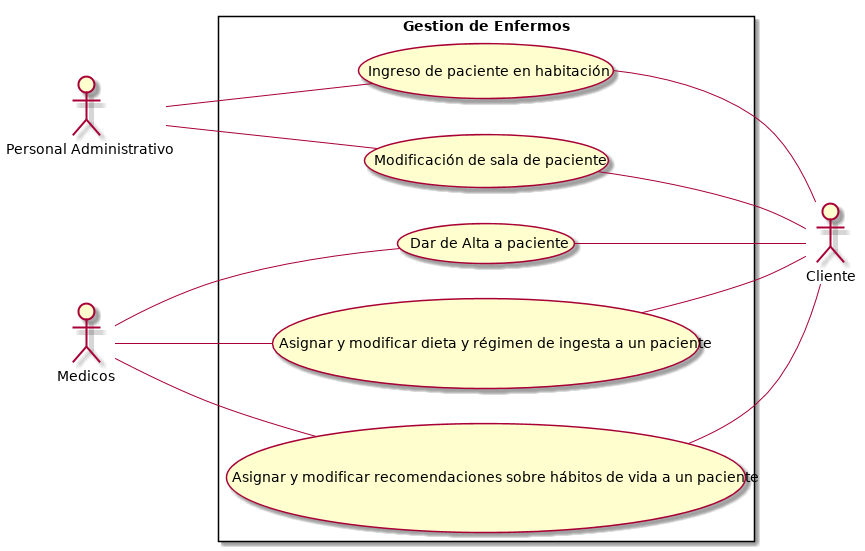
\includegraphics[scale=0.4]{GestionDeEnfermos}\\
	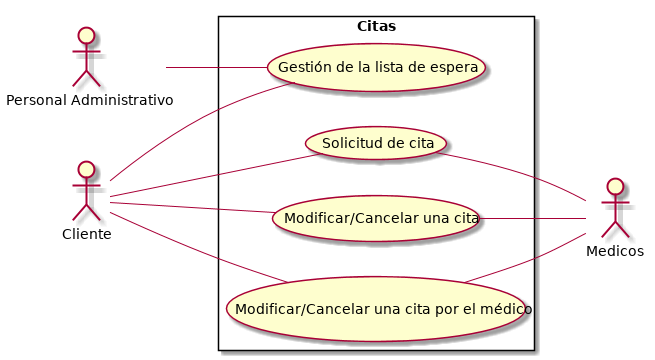
\includegraphics[scale=0.5]{GestionDeCitas}\\
	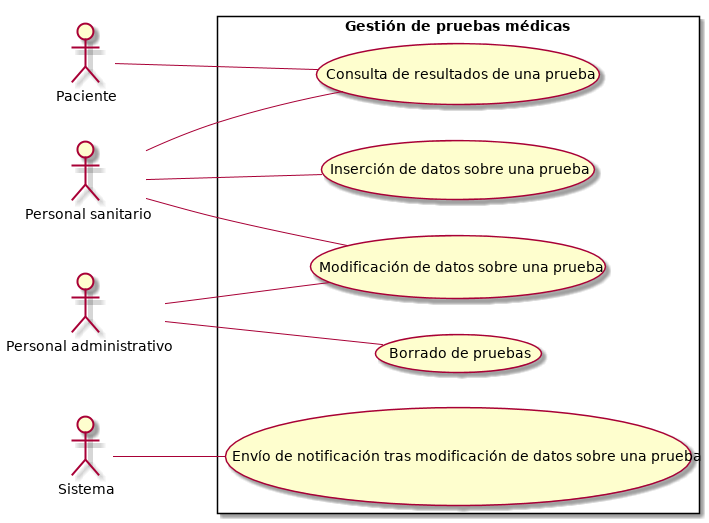
\includegraphics[scale=0.4]{gestion-de-pruebas-medicas}\\
	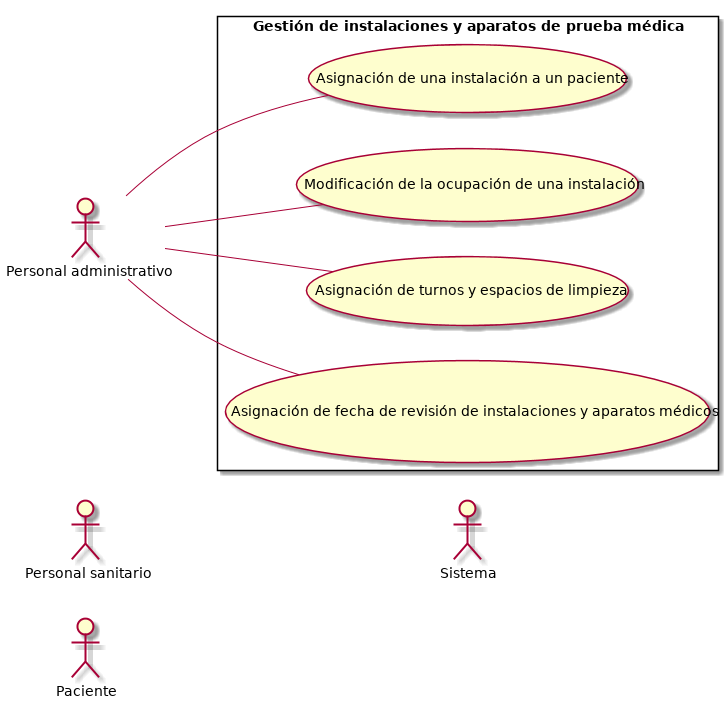
\includegraphics[scale=0.4]{gestion-instalaciones-y-aparatos}\\
	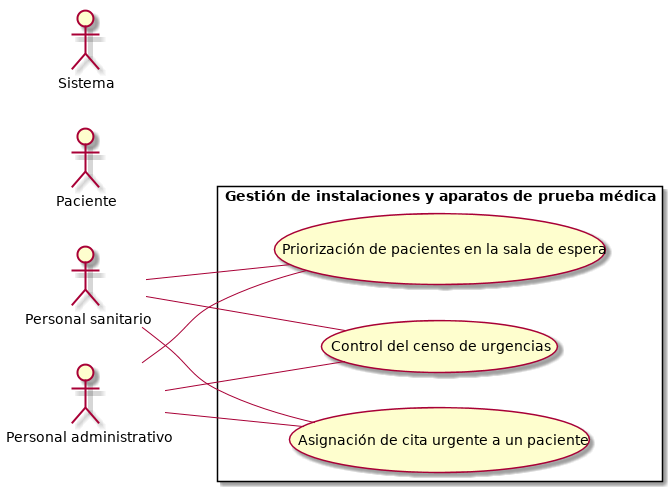
\includegraphics[scale=0.4]{gestion-servicios-urgencia}\\
	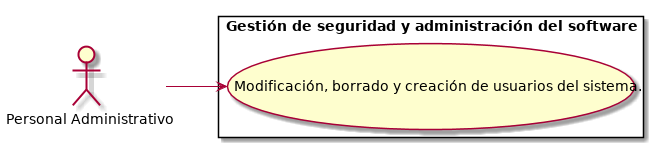
\includegraphics[scale=0.5]{Gestion_de_seguridad_y_administracion_del_software}\\
	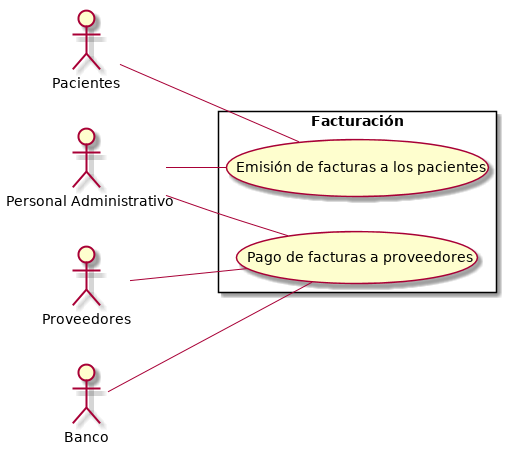
\includegraphics[scale=0.5]{Facturacion}\\
	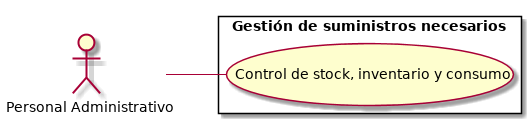
\includegraphics[scale=0.5]{Gestion_de_suministros_necesarios}\\
	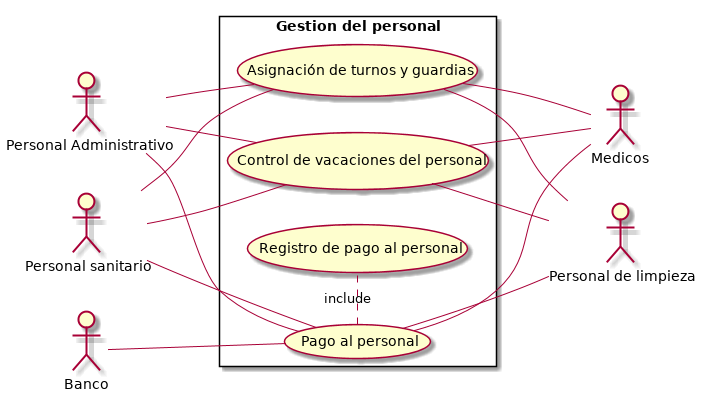
\includegraphics[scale=0.5]{Gestion_del_personal}\\
\end{center}


\section*{Descripción de los actores.}

Han aparecido una serie de actores en nuestros diagramas de casos de uso. Su descripción detallada es la siguiente:

%%FIXME:Primer grupo de tablas
  %%%%%%%%%%%%%%%%%%%%%%%%%%%%%%  1  %%%%%%%%%%%%%%%%%%%%%%%%%%%%%%%%%%%%
  \begin{tabular}{|>{\raggedright}p{58pt}|>{\raggedright}p{109pt}|>{\raggedright}p{1pt}|>{\raggedright}p{17pt}|>{\raggedright}p{28pt}|>{\raggedright}p{0pt}|>{\raggedright}p{18pt}|>{\raggedright}p{20pt}|}

	\hline
  %Actor e Identificador
	\textbf{Actor} & \multicolumn{5}{p{155pt}|}{Personal}	& \multicolumn{2}{p{39pt}|}{\textbf{AP-0}}\tabularnewline

	\hline
  %Descripcion
	\textbf{Descripción} & \multicolumn{7}{p{265pt}|}{Clase padre de AP-1,AP-2 y AP-3}\tabularnewline

	\hline
  %Caracteristicas
	\textbf{Características} & \multicolumn{7}{p{265pt}|}{Los atributos en común que contienen todos los trabajadores del hospital, están contenidos dentro de esta.}\tabularnewline

	\hline
  %Relaciones
	\textbf{Relaciones} & \multicolumn{7}{p{265pt}|}{AP-1,AP-2, AP-3 y AP-4 son hijos de este.}\tabularnewline
	\hline
  %Referencias
	\textbf{Referencias} & \multicolumn{7}{p{265pt}|}{Como tal no aparece en ningún diagrama ni caso de uso. Sus hijos, sin embargo, sí.}\tabularnewline
	\hline
  %Autor, Fecha y Versión
	\textbf{Autor} & Grupo 9  & \multicolumn{2}{p{30pt}|}{
	\textbf{Fecha}} & 1/4/18 & \multicolumn{2}{p{30pt}|}{
	\textbf{Versión}} & 1.0 \tabularnewline
	\hline
	\end{tabular}


	\vspace{0.5cm}	\begin{tabular}{|>{\raggedright}p{61pt}|>{\raggedright}p{190pt}|>{\raggedright}p{61pt}|}
	\hline
  %Atributos
	 \multicolumn{3}{|p{313pt}|}{
	\textbf{Atributos}}\tabularnewline
	\hline
  %Nombre, Descripción y Tipo
	\textbf{Nombre}  & \textbf{Descripción} & \textbf{Tipo}\tabularnewline
	\hline
ID & Identificador único y personal de cada trabajador. A partir de este se localizan todos sus datos en las distintas tablas que se vayan creando. & String \tabularnewline
	\hline
Trabajadores & Puntero a la base de datos que contiene toda la información de nuestros trabajadores. & BaseDatos\tabularnewline
	\hline
Equipo & Puntero a la base de datos que contiene toda la información de la maquinaria y suministros & BaseDatos\tabularnewline
	\hline

	\end{tabular}

	\vspace{0.5cm}
	\begin{tabular}{|>{\raggedright}p{337pt}|}
	\hline
  %Comentarios
	\textbf{Comentarios}\tabularnewline
	\hline
	Apartir del ID, podremos acceder a toda la información necesaria para nuestro personal, sea cual sea la base de datos en la que esté almacenada. Por ello no es necesario de más campos para los distintos datos y detalles del personal, pues estos estarían correctamente almacenados en las bases de datos y serían modificadas en los distintos métodos.
	Así mismo, cabe mencionar que con el tiempo puede verse la idea de juntar las bases de datos en una sóla o crear nuevas.
\tabularnewline
	\hline
	\end{tabular}
	
	
	\vspace{2.0cm}
	%%FIXME:Segundo grupo de tablas
  %%%%%%%%%%%%%%%%%%%%%%%%%%%%%%  1  %%%%%%%%%%%%%%%%%%%%%%%%%%%%%%%%%%%%
  \begin{tabular}{|>{\raggedright}p{58pt}|>{\raggedright}p{109pt}|>{\raggedright}p{1pt}|>{\raggedright}p{17pt}|>{\raggedright}p{28pt}|>{\raggedright}p{0pt}|>{\raggedright}p{18pt}|>{\raggedright}p{20pt}|}

	\hline
  %Actor e Identificador
	\textbf{Actor} & \multicolumn{5}{p{155pt}|}{Personal Médico}	& \multicolumn{2}{p{39pt}|}{\textbf{AP-1}}\tabularnewline

	\hline
  %Descripcion
	\textbf{Descripción} & \multicolumn{7}{p{265pt}|}{Se encarga de atender correctamente a los pacientes, así como controlar y modificar algunos datos de este relacionados con su tratamiento.}\tabularnewline

	\hline
  %Caracteristicas
	\textbf{Características} & \multicolumn{7}{p{265pt}|}{Alto conocimiento médico y con cierto grado de autoridad.}\tabularnewline

	\hline
  %Relaciones
	\textbf{Relaciones} & \multicolumn{7}{p{265pt}|}{Atiende a los pacientes, así como coopera con el personal admistrativo. Hereda de AP-0.}\tabularnewline
	\hline
  %Referencias
	\textbf{Referencias} & \multicolumn{7}{p{265pt}|}{Gestión del Personal; Gestión de Citas; Gestión de Enfermos.}\tabularnewline
	\hline
  %Autor, Fecha y Versión
	\textbf{Autor} & Grupo 9  & \multicolumn{2}{p{30pt}|}{
	\textbf{Fecha}} & 1/4/18 & \multicolumn{2}{p{30pt}|}{
	\textbf{Versión}} & 1.0 \tabularnewline
	\hline
	\end{tabular}


	\vspace{0.5cm}	\begin{tabular}{|>{\raggedright}p{61pt}|>{\raggedright}p{190pt}|>{\raggedright}p{61pt}|}
	\hline
  %Atributos
	 \multicolumn{3}{|p{313pt}|}{
	\textbf{Atributos}}\tabularnewline
	\hline
  %Nombre, Descripción y Tipo
	\textbf{Nombre}  & \textbf{Descripción} & \textbf{Tipo}\tabularnewline
	\hline
Pacientes & Puntero a la base de datos que contiene toda la información de nuestros pacientes. & BaseDatos\tabularnewline
	\hline
	\end{tabular}

	\vspace{0.5cm}
	\begin{tabular}{|>{\raggedright}p{337pt}|}
	\hline
  %Comentarios
	\textbf{Comentarios}\tabularnewline
	\hline
	Comentarios adicionales sobre el actor \tabularnewline
	\hline
	\end{tabular}
	
	\vspace{2.0cm}
	%%FIXME:Tercer grupo de tablas
  %%%%%%%%%%%%%%%%%%%%%%%%%%%%%%  1  %%%%%%%%%%%%%%%%%%%%%%%%%%%%%%%%%%%%
  \begin{tabular}{|>{\raggedright}p{58pt}|>{\raggedright}p{109pt}|>{\raggedright}p{1pt}|>{\raggedright}p{17pt}|>{\raggedright}p{28pt}|>{\raggedright}p{0pt}|>{\raggedright}p{18pt}|>{\raggedright}p{20pt}|}

	\hline
  %Actor e Identificador
	\textbf{Actor} & \multicolumn{5}{p{155pt}|}{Personal Sanitario}	& \multicolumn{2}{p{39pt}|}{\textbf{AP-2}}\tabularnewline

	\hline
  %Descripcion
	\textbf{Descripción} & \multicolumn{7}{p{265pt}|}{Sigue las intrucciones del médico en cuanto al cuidado del paciente. }\tabularnewline

	\hline
  %Caracteristicas
	\textbf{Características} & \multicolumn{7}{p{265pt}|}{Conocimiento médico variable según al puesto concreto que ocupe. Por lo general, carece de permisos más allá de lectura. }\tabularnewline

	\hline
  %Relaciones
	\textbf{Relaciones} & \multicolumn{7}{p{265pt}|}{Siguen instrucciones de los distintos médicos, así como indicarse entre ellos mismos según su trabajo concreto. Hereda de AP-0.}\tabularnewline
	\hline
  %Referencias
	\textbf{Referencias} & \multicolumn{7}{p{265pt}|}{Gestión del personal; Gestión de Urgencias; Gestión de Instalaciones y Aparatos; Gestión de Pruebas Médicas.}\tabularnewline
	\hline
  %Autor, Fecha y Versión
	\textbf{Autor} & Grupo 9  & \multicolumn{2}{p{30pt}|}{
	\textbf{Fecha}} & 1/4/18 & \multicolumn{2}{p{30pt}|}{
	\textbf{Versión}} & 1.0 \tabularnewline
	\hline
	\end{tabular}


	\vspace{0.5cm}	\begin{tabular}{|>{\raggedright}p{61pt}|>{\raggedright}p{190pt}|>{\raggedright}p{61pt}|}
	\hline
  %Atributos
	 \multicolumn{3}{|p{313pt}|}{
	\textbf{Atributos}}\tabularnewline
	\hline
  %Nombre, Descripción y Tipo
	\textbf{Nombre}  & \textbf{Descripción} & \textbf{Tipo}\tabularnewline
	\hline
Pacientes & Puntero a la base de datos que contiene toda la información de nuestros pacientes. & BaseDatos\tabularnewline
	\hline

	\end{tabular}

	\vspace{0.5cm}
	\begin{tabular}{|>{\raggedright}p{337pt}|}
	\hline
  %Comentarios
	\textbf{Comentarios}\tabularnewline
	\hline
	Comentarios adicionales sobre el actor \tabularnewline
	\hline
	\end{tabular}
	
		\vspace{2.0cm}
	%%FIXME:Cuarto grupo de tablas
  %%%%%%%%%%%%%%%%%%%%%%%%%%%%%%  1  %%%%%%%%%%%%%%%%%%%%%%%%%%%%%%%%%%%%
  \begin{tabular}{|>{\raggedright}p{58pt}|>{\raggedright}p{109pt}|>{\raggedright}p{1pt}|>{\raggedright}p{17pt}|>{\raggedright}p{28pt}|>{\raggedright}p{0pt}|>{\raggedright}p{18pt}|>{\raggedright}p{20pt}|}

	\hline
  %Actor e Identificador
	\textbf{Actor} & \multicolumn{5}{p{155pt}|}{Personal Administrativo}	& \multicolumn{2}{p{39pt}|}{\textbf{AP-3}}\tabularnewline

	\hline
  %Descripcion
	\textbf{Descripción} & \multicolumn{7}{p{265pt}|}{Se encarga de gestionar todos datos del paciente, así como también los recursos del hospital.}\tabularnewline

	\hline
  %Caracteristicas
	\textbf{Características} & \multicolumn{7}{p{265pt}|}{No necesita de conocimiento médico para desempeñar su labor. Posee permisos de gestión, pero no puede modificar ningún dato médico de ningún paciente.}\tabularnewline

	\hline
  %Relaciones
	\textbf{Relaciones} & \multicolumn{7}{p{265pt}|}{Coopera con todos los actores.Hereda de AP-0.}\tabularnewline
	\hline
  %Referencias
	\textbf{Referencias} & \multicolumn{7}{p{265pt}|}{Gestión del personal; Facturación; Gestión de Citas; Gestión de Enfermos; Gestión de Seguridad y Administración del Software; Gestión de Suministros; Gestión de Servicios de Urgencia; Gestión de Pruebas Médicas; Gestión de Instalaciones y Aparatos.}\tabularnewline
	\hline
  %Autor, Fecha y Versión
	\textbf{Autor} & Grupo 9  & \multicolumn{2}{p{30pt}|}{
	\textbf{Fecha}} & 1/4/18 & \multicolumn{2}{p{30pt}|}{
	\textbf{Versión}} & 1.0 \tabularnewline
	\hline
	\end{tabular}


	\vspace{0.5cm}	\begin{tabular}{|>{\raggedright}p{61pt}|>{\raggedright}p{190pt}|>{\raggedright}p{61pt}|}
	\hline
  %Atributos
	 \multicolumn{3}{|p{313pt}|}{
	\textbf{Atributos}}\tabularnewline
	\hline
  %Nombre, Descripción y Tipo
	\textbf{Nombre}  & \textbf{Descripción} & \textbf{Tipo}\tabularnewline
	\hline
Pacientes & Puntero a la base de datos que contiene toda la información de nuestros pacientes. & BaseDatos\tabularnewline
	\hline

	\end{tabular}

	\vspace{0.5cm}
	\begin{tabular}{|>{\raggedright}p{337pt}|}
	\hline
  %Comentarios
	\textbf{Comentarios}\tabularnewline
	\hline
El grado de interacción con cada uno de los actores depende de su puesto asignado,que puede ser variable según el momento y necesidades del hospital, y este no afecta a sus permisos al sistema.
 \tabularnewline
	\hline
	\end{tabular}
	
	\vspace{2.0cm}
	
		%%FIXME:Quinto grupo de tablas
  %%%%%%%%%%%%%%%%%%%%%%%%%%%%%%  1  %%%%%%%%%%%%%%%%%%%%%%%%%%%%%%%%%%%%
  \begin{tabular}{|>{\raggedright}p{58pt}|>{\raggedright}p{109pt}|>{\raggedright}p{1pt}|>{\raggedright}p{17pt}|>{\raggedright}p{28pt}|>{\raggedright}p{0pt}|>{\raggedright}p{18pt}|>{\raggedright}p{20pt}|}

	\hline
  %Actor e Identificador
	\textbf{Actor} & \multicolumn{5}{p{155pt}|}{Personal de Limpieza}	& \multicolumn{2}{p{39pt}|}{\textbf{AP-4}}\tabularnewline

	\hline
  %Descripcion
	\textbf{Descripción} & \multicolumn{7}{p{265pt}|}{Se encarga de que las instalaciones estén en perfecto estado de desinfección.}\tabularnewline

	\hline
  %Caracteristicas
	\textbf{Características} & \multicolumn{7}{p{265pt}|}{No necesita de conocimiento médico para desempeñar su labor. Únicamente puede accceder a sus propios datos personales y consultar sus datos laborales.}\tabularnewline

	\hline
  %Relaciones
	\textbf{Relaciones} & \multicolumn{7}{p{265pt}|}{Coopera con todos los actores.Hereda de AP-0.}\tabularnewline
	\hline
  %Referencias
	\textbf{Referencias} & \multicolumn{7}{p{265pt}|}{Gestión del personal.}\tabularnewline
	\hline
  %Autor, Fecha y Versión
	\textbf{Autor} & Grupo 9  & \multicolumn{2}{p{30pt}|}{
	\textbf{Fecha}} & 1/4/18 & \multicolumn{2}{p{30pt}|}{
	\textbf{Versión}} & 1.0 \tabularnewline
	\hline
	\end{tabular}

	\vspace{0.5cm}
	\begin{tabular}{|>{\raggedright}p{337pt}|}
	\hline
  %Comentarios
	\textbf{Comentarios}\tabularnewline
	\hline
De primeras no requiere de ningún Atributo extra más allá de los proporcionados por AP-0.
 \tabularnewline
	\hline
	\end{tabular}
	
	\vspace{2.0cm}
	
%%FIXME:Sexto grupo de tablas
	
	\begin{tabular}{|>{\raggedright}p{58pt}|>{\raggedright}p{109pt}|>{\raggedright}p{1pt}|>{\raggedright}p{17pt}|>{\raggedright}p{28pt}|>{\raggedright}p{0pt}|>{\raggedright}p{18pt}|>{\raggedright}p{20pt}|}

	\hline
  %Actor e Identificador
	\textbf{Actor} & \multicolumn{5}{p{155pt}|}{Paciente ó Cliente}	& \multicolumn{2}{p{39pt}|}{\textbf{AC}}\tabularnewline

	\hline
  %Descripcion
	\textbf{Descripción} & \multicolumn{7}{p{265pt}|}{Padece alguna enfermedad y necesita ser atendido por nuestro personal.}\tabularnewline

	\hline
  %Caracteristicas
	\textbf{Características} & \multicolumn{7}{p{265pt}|}{Por lo general, carece de conocimiento médico y tampoco posee permisos salvo modificar sus propios datos personales.}\tabularnewline

	\hline
  %Relaciones
	\textbf{Relaciones} & \multicolumn{7}{p{265pt}|}{Es atendido por el personal médico y el personal administrativo mantiene actualizados sus datos.}\tabularnewline
	\hline
  %Referencias
	\textbf{Referencias} & \multicolumn{7}{p{265pt}|}{Facturación; Gestión de Citas; Gestión de Enfermos; Gestión de Servicios de Urgencia; Gestión de Pruebas Médicas; Gestión de Instalaciones y Aparatos.}\tabularnewline
	\hline
  %Autor, Fecha y Versión
	\textbf{Autor} & Grupo 9  & \multicolumn{2}{p{30pt}|}{
	\textbf{Fecha}} & 1/4/18 & \multicolumn{2}{p{30pt}|}{
	\textbf{Versión}} & 1.0 \tabularnewline
	\hline
	\end{tabular}


	\vspace{0.5cm}	\begin{tabular}{|>{\raggedright}p{61pt}|>{\raggedright}p{190pt}|>{\raggedright}p{61pt}|}
	\hline
  %Atributos
	 \multicolumn{3}{|p{313pt}|}{
	\textbf{Atributos}}\tabularnewline
	\hline
  %Nombre, Descripción y Tipo
	\textbf{Nombre}  & \textbf{Descripción} & \textbf{Tipo}\tabularnewline
	\hline
	 ID & Identificador único y personal de cada paciente. A partir de este se localizan todos sus datos en las distintas tablas que se vayan creando. & String \tabularnewline
	\hline
Pacientes & Puntero a la base de datos que contiene toda la información de nuestros pacientes. & BaseDatos\tabularnewline
	\hline

	\end{tabular}

	\vspace{0.5cm}
	\begin{tabular}{|>{\raggedright}p{337pt}|}
	\hline
  %Comentarios
	\textbf{Comentarios}\tabularnewline
	\hline
	Cuando indicamos que puede modificar sus propios datos personales, nos referimos datos como su dirección actual o número de teléfono. Por supuesto, los datos relacionados estrictamente con su salud no pueden ser modificados por el paciente.\tabularnewline
	\hline
	\end{tabular}
	
	
	\vspace{2.0cm}
	%%FIXME:Séptimo grupo de tablas
	
	\begin{tabular}{|>{\raggedright}p{58pt}|>{\raggedright}p{109pt}|>{\raggedright}p{1pt}|>{\raggedright}p{17pt}|>{\raggedright}p{28pt}|>{\raggedright}p{0pt}|>{\raggedright}p{18pt}|>{\raggedright}p{20pt}|}

	\hline
  %Actor e Identificador
	\textbf{Actor} & \multicolumn{5}{p{155pt}|}{Banco}	& \multicolumn{2}{p{39pt}|}{\textbf{AB}}\tabularnewline

	\hline
  %Descripcion
	\textbf{Descripción} & \multicolumn{7}{p{265pt}|}{Intermediario entre nuestro hospital y el paciente para el tema monetario.}\tabularnewline

	\hline
  %Caracteristicas
	\textbf{Características} & \multicolumn{7}{p{265pt}|}{Se trata de una entidad por sí misma, gracias a ella se gestiona más cómodamente el dinero del hospital.}\tabularnewline

	\hline
  %Relaciones
	\textbf{Relaciones} & \multicolumn{7}{p{265pt}|}{Los pacientes pagan a través de este, ya sea por ingreso o transferencia bancaria,}\tabularnewline
	\hline
  %Referencias
	\textbf{Referencias} & \multicolumn{7}{p{265pt}|}{Facturación; Gestión del Personal.}\tabularnewline
	\hline
  %Autor, Fecha y Versión
	\textbf{Autor} & Grupo 9  & \multicolumn{2}{p{30pt}|}{
	\textbf{Fecha}} & 1/4/18 & \multicolumn{2}{p{30pt}|}{
	\textbf{Versión}} & 1.0 \tabularnewline
	\hline
	\end{tabular}


	\vspace{0.5cm}
	\begin{tabular}{|>{\raggedright}p{337pt}|}
	\hline
  %Comentarios
	\textbf{Comentarios}\tabularnewline
	\hline
	Carece de atributos porque no es una entidad que nosotros programemos, sino una con la que colaboramos y utilizamos sus recursos para algunas prestaciones de nuestra aplicación.\tabularnewline
	\hline
	\end{tabular}
	
	
	\vspace{2.0cm}


	
	%%FIXME:Octavo grupo de tablas
	
	\begin{tabular}{|>{\raggedright}p{58pt}|>{\raggedright}p{109pt}|>{\raggedright}p{1pt}|>{\raggedright}p{17pt}|>{\raggedright}p{28pt}|>{\raggedright}p{0pt}|>{\raggedright}p{18pt}|>{\raggedright}p{20pt}|}

	\hline
  %Actor e Identificador
	\textbf{Actor} & \multicolumn{5}{p{155pt}|}{Proveedores}	& \multicolumn{2}{p{39pt}|}{\textbf{APS}}\tabularnewline

	\hline
  %Descripcion
	\textbf{Descripción} & \multicolumn{7}{p{265pt}|}{Son los encargados de, a partir de los pedidos, traer los suministros necesarios para el hospital.}\tabularnewline

	\hline
  %Caracteristicas
	\textbf{Características} & \multicolumn{7}{p{265pt}|}{Conjunto de varias entidades que nos proporcionan los recursos solicitados, recibiendo dinero a cambio. Además, deben de ofrecer un servicio de garantía por si algo falla.}\tabularnewline

	\hline
  %Relaciones
	\textbf{Relaciones} & \multicolumn{7}{p{265pt}|}{Se relacionan sobre todo con el personal administrativo, el banco y, a veces, con los médicos. Con estos últimos lo hacen para ofrecerles productos. }\tabularnewline
	\hline
  %Referencias
	\textbf{Referencias} & \multicolumn{7}{p{265pt}|}{Facturación.}\tabularnewline
	\hline
  %Autor, Fecha y Versión
	\textbf{Autor} & Grupo 9  & \multicolumn{2}{p{30pt}|}{
	\textbf{Fecha}} & 1/4/18 & \multicolumn{2}{p{30pt}|}{
	\textbf{Versión}} & 1.0 \tabularnewline
	\hline
	\end{tabular}


	\vspace{0.5cm}
	\begin{tabular}{|>{\raggedright}p{337pt}|}
	\hline
  %Comentarios
	\textbf{Comentarios}\tabularnewline
	\hline
	Carece de atributos porque no son entidades que nosotros programemos, sino que colaboramos con ellas y utilizamos su información para mantener actualizadas las distintas bases de datos.\tabularnewline
	\hline
	\end{tabular}
	
	
	\vspace{2.0cm}
	
	\section*{Descripción de casos de uso}
	Una vez que tenemos los actores y los diagramas de casos de uso, pasamos a describir todos los casos de uso de forma completa:
	
	

	
	
		\begin{tabular}{|>{\raggedright}p{58pt}|>{\raggedright}p{109pt}|>{\raggedright}p{1pt}|>{\raggedright}p{17pt}|>{\raggedright}p{28pt}|>{\raggedright}p{0pt}|>{\raggedright}p{18pt}|>{\raggedright}p{20pt}|}
	\hline
	 \textbf{Caso de Uso} &

	%Nombre del CU e identificador
	\multicolumn{5}{p{155pt}|}{Permitir ingresar paciente en cama/habitación}	& \multicolumn{2}{p{39pt}|}{\textbf{CU1}}\tabularnewline

	\hline

	%Listado de actores
	\textbf{Actores} & \multicolumn{7}{p{194pt}|}{Cliente, Personal Administrativo}\tabularnewline
	\hline

	%Tipo de CU
	\textbf{Tipo} & \multicolumn{7}{p{194pt}|}{Primario}\tabularnewline
	\hline

	%Requisitos del CU
	\textbf{Referencias} & \multicolumn{2}{p{110pt}|}{} & \multicolumn{5}{p{84pt}|}{Modificar habitación/cama del cliente}\tabularnewline
	\hline

	%Precondiciones
	\textbf{Precondición} & \multicolumn{7}{p{194pt}|}{El cliente debe padecer alguna enfermedad y debe haber espacio libre}\tabularnewline
	\hline

	%Postcondiciones
	\textbf{Postcondición} & \multicolumn{7}{p{194pt}|}{El cliente tendrá asignada una habitación y habrá una habitación libre menos}\tabularnewline
	\hline

	%Autor y fecha
	\textbf{Autor} & Grupo 9 & \multicolumn{2}{p{30pt}|}{
	\textbf{Fecha}} & 8 Abril & \multicolumn{2}{p{30pt}|}{
	\textbf{Versión}} & 1.0 \tabularnewline
	\hline
	\end{tabular}

	\vspace{0.5cm}

	%Proposito
	\begin{tabular}{|>{\raggedright}p{337pt}|}
		\hline
		\textbf{Proposito} \tabularnewline \hline
			Dar una habitación a un cliente que la solicita o la necesita
		\tabularnewline
		\hline
	\end{tabular}

	\vspace{0.5cm}
	%Resumen
	\begin{tabular}{|>{\raggedright}p{337pt}|}
		\hline
		\textbf{Resumen}\tabularnewline
		\hline
			El cliente o alguna persona en nombre del cliente solicitará una habitación, el personal administrativo solicitará al sistema que se le asigne una habitación al paciente , el sistema buscará esta habitación y se la comunicará al personal.
		\tabularnewline
		\hline
	\end{tabular}
	\vspace{0.5cm}
	
	
	\begin{tabular}{|>{\raggedright}p{58pt}|>{\raggedright}p{109pt}|>{\raggedright}p{1pt}|>{\raggedright}p{17pt}|>{\raggedright}p{28pt}|>{\raggedright}p{0pt}|>{\raggedright}p{18pt}|>{\raggedright}p{20pt}|}
	\hline
	 \textbf{Caso de Uso} &

	%Nombre del CU e identificador
	\multicolumn{5}{p{155pt}|}{Modificar sala del cliente}	& \multicolumn{2}{p{39pt}|}{\textbf{CU2}}\tabularnewline

	\hline

	%Listado de actores
	\textbf{Actores} & \multicolumn{7}{p{194pt}|}{Cliente/Médico, Personal administrativo}\tabularnewline
	\hline

	%Tipo de CU
	\textbf{Tipo} & \multicolumn{7}{p{194pt}|}{Secundario}\tabularnewline
	\hline

	%Requisitos del CU
	\textbf{Referencias} & \multicolumn{2}{p{110pt}|}{Que el cliente esté ya en una sala} & \multicolumn{5}{p{84pt}|}{}\tabularnewline
	\hline

	%Precondiciones
	\textbf{Precondición} & \multicolumn{7}{p{194pt}|}{Se necesita que el cliente siga enfermo, que haya salas disponibles y que el cliente esté ya en una sala}\tabularnewline
	\hline

	%Postcondiciones
	\textbf{Postcondición} & \multicolumn{7}{p{194pt}|}{Que la habitación anterior quede libre, y haya otra diferente ocupada}\tabularnewline
	\hline

	%Autor y fecha
	\textbf{Autor} & Grupo 9 & \multicolumn{2}{p{30pt}|}{
	\textbf{Fecha}} & 8 Abril & \multicolumn{2}{p{30pt}|}{
	\textbf{Versión}} & 1.0 \tabularnewline
	\hline
	\end{tabular}

	\vspace{0.5cm}

	%Proposito
	\begin{tabular}{|>{\raggedright}p{337pt}|}
		\hline
		\textbf{Proposito} \tabularnewline \hline
			Cambiar de habitación a paciente
		\tabularnewline
		\hline
	\end{tabular}

	\vspace{0.5cm}
	%Resumen
	\begin{tabular}{|>{\raggedright}p{337pt}|}
		\hline
		\textbf{Resumen}\tabularnewline
		\hline
			Se solicitará por motivo justificado que a un cliente se le cambie la habitación en la que está. El personal administrativo le pedirá al sistema que lo haga y el sistema hará la labor de dejar la sala anterior libre, buscar una nueva y comunicarla al personal administrativo.
		\tabularnewline
		\hline
	\end{tabular}
	\vspace{0.5cm}


	\begin{tabular}{|>{\raggedright}p{58pt}|>{\raggedright}p{109pt}|>{\raggedright}p{1pt}|>{\raggedright}p{17pt}|>{\raggedright}p{28pt}|>{\raggedright}p{0pt}|>{\raggedright}p{18pt}|>{\raggedright}p{20pt}|}
	\hline
	 \textbf{Caso de Uso} &

	%Nombre del CU e identificador
	\multicolumn{5}{p{155pt}|}{Permitir dar de alta a un paciente ingresado}	& \multicolumn{2}{p{39pt}|}{\textbf{CU3}}\tabularnewline

	\hline

	%Listado de actores
	\textbf{Actores} & \multicolumn{7}{p{194pt}|}{Médico}\tabularnewline
	\hline

	%Tipo de CU
	\textbf{Tipo} & \multicolumn{7}{p{194pt}|}{Primario, Esencial}\tabularnewline
	\hline

	%Requisitos del CU
	\textbf{Referencias} & \multicolumn{2}{p{110pt}|}{Indicamos que requisitos se pueden incluir dentro} & \multicolumn{5}{p{84pt}|}{CU que tienen relación con este}\tabularnewline
	\hline

	%Precondiciones
	\textbf{Precondición} & \multicolumn{7}{p{194pt}|}{El paciente debe estar ingresado y con una habitación asignada}\tabularnewline
	\hline

	%Postcondiciones
	\textbf{Postcondición} & \multicolumn{7}{p{194pt}|}{El paciente ya no estará en el sistema como enfermo, y habrá una habitación libre más.}\tabularnewline
	\hline

	%Autor y fecha
	\textbf{Autor} & Grupo 9 & \multicolumn{2}{p{30pt}|}{
	\textbf{Fecha}} & 8 Abril & \multicolumn{2}{p{30pt}|}{
	\textbf{Versión}} & 1.0 \tabularnewline
	\hline
	\end{tabular}

	\vspace{0.5cm}

	%Proposito
	\begin{tabular}{|>{\raggedright}p{337pt}|}
		\hline
		\textbf{Proposito} \tabularnewline \hline
			Indicar que el paciente ya no está en el hospital
		\tabularnewline
		\hline
	\end{tabular}

	\vspace{0.5cm}
	%Resumen
	\begin{tabular}{|>{\raggedright}p{337pt}|}
		\hline
		\textbf{Resumen}\tabularnewline
		\hline
			El médico, tras comprobar que el paciente puede irse, indicará al sistema que eliminte al paciente de los pacientes que están en ese momento en el hospital. El sistema eliminará al paciente de esta lista y marcará la sala en la que estaba el paciente como "libre".
		\tabularnewline
		\hline
	\end{tabular}
	\vspace{0.5cm}


	\begin{tabular}{|>{\raggedright}p{58pt}|>{\raggedright}p{109pt}|>{\raggedright}p{1pt}|>{\raggedright}p{17pt}|>{\raggedright}p{28pt}|>{\raggedright}p{0pt}|>{\raggedright}p{18pt}|>{\raggedright}p{20pt}|}
	\hline
	 \textbf{Caso de Uso} &

	%Nombre del CU e identificador
	\multicolumn{5}{p{155pt}|}{Asignar/Modificar Dieta-medicamentos-régimen de ingesta a paciente}	& \multicolumn{2}{p{39pt}|}{\textbf{CU4-5}}\tabularnewline

	\hline

	%Listado de actores
	\textbf{Actores} & \multicolumn{7}{p{194pt}|}{Médico}\tabularnewline
	\hline

	%Tipo de CU
	\textbf{Tipo} & \multicolumn{7}{p{194pt}|}{Secundario}\tabularnewline
	\hline

	%Requisitos del CU
	\textbf{Referencias} & \multicolumn{2}{p{110pt}|}{Puede que el paciente ya tenga una dieta asignada} & \multicolumn{5}{p{84pt}|}{}\tabularnewline
	\hline

	%Precondiciones
	\textbf{Precondición} & \multicolumn{7}{p{194pt}|}{El paciente deberá estar con una sala asignada y marcado en su ficha como "enfermo actualmente"}\tabularnewline
	\hline

	%Postcondiciones
	\textbf{Postcondición} & \multicolumn{7}{p{194pt}|}{En la ficha del paciente estará la dieta-medicamentos asignados al paciente para que este o el médico puedan consultarlos}\tabularnewline
	\hline

	%Autor y fecha
	\textbf{Autor} & Grupo 9 & \multicolumn{2}{p{30pt}|}{
	\textbf{Fecha}} & 8 Abril & \multicolumn{2}{p{30pt}|}{
	\textbf{Versión}} & 1.0 \tabularnewline
	\hline
	\end{tabular}

	\vspace{0.5cm}

	%Proposito
	\begin{tabular}{|>{\raggedright}p{337pt}|}
		\hline
		\textbf{Proposito} \tabularnewline \hline
			Se pretende que el paciente y el médico tengan guardada la información sobre la dieta-medicamentos-régimen que debe seguir el paciente
		\tabularnewline
		\hline
	\end{tabular}

	\vspace{0.5cm}
	%Resumen
	\begin{tabular}{|>{\raggedright}p{337pt}|}
		\hline
		\textbf{Resumen}\tabularnewline
		\hline
			El médico introducirá en el sistema los datos que crea convenientes para el paciente y el sistema los asignará a la ficha del paciente, para mostrarlos cuando sea necesario.
		\tabularnewline
		\hline
	\end{tabular}
	\vspace{0.5cm}


	\begin{tabular}{|>{\raggedright}p{58pt}|>{\raggedright}p{109pt}|>{\raggedright}p{1pt}|>{\raggedright}p{17pt}|>{\raggedright}p{28pt}|>{\raggedright}p{0pt}|>{\raggedright}p{18pt}|>{\raggedright}p{20pt}|}
	\hline
	 \textbf{Caso de Uso} &

	%Nombre del CU e identificador
	\multicolumn{5}{p{155pt}|}{Asignar hábitos de vida la paciente}	& \multicolumn{2}{p{39pt}|}{\textbf{CU6}}\tabularnewline

	\hline

	%Listado de actores
	\textbf{Actores} & \multicolumn{7}{p{194pt}|}{Médico}\tabularnewline
	\hline

	%Tipo de CU
	\textbf{Tipo} & \multicolumn{7}{p{194pt}|}{Opcional}\tabularnewline
	\hline

	%Requisitos del CU
	\textbf{Referencias} & \multicolumn{2}{p{110pt}|}{El paciente puede tener asignados dieta-régimen de ingesta-medicamentos} & \multicolumn{5}{p{84pt}|}{Asignar/Modificar medicamentos-régimen de ingesta-dieta a paciente}\tabularnewline
	\hline

	%Precondiciones
	\textbf{Precondición} & \multicolumn{7}{p{194pt}|}{El paciente debe estar en el sistema y puede que se le haya dado el alta}\tabularnewline
	\hline

	%Postcondiciones
	\textbf{Postcondición} & \multicolumn{7}{p{194pt}|}{En la ficha del paciente habrá algunos hábitos de vida recomendados}\tabularnewline
	\hline

	%Autor y fecha
	\textbf{Autor} & Grupo 9 & \multicolumn{2}{p{30pt}|}{
	\textbf{Fecha}} & 8 Abril & \multicolumn{2}{p{30pt}|}{
	\textbf{Versión}} & 1.0 \tabularnewline
	\hline
	\end{tabular}

	\vspace{0.5cm}

	%Proposito
	\begin{tabular}{|>{\raggedright}p{337pt}|}
		\hline
		\textbf{Proposito} \tabularnewline \hline
			Guardar en la ficha del paciente hábitos de vida recomendados para el mismo.
		\tabularnewline
		\hline
	\end{tabular}

	\vspace{0.5cm}
	%Resumen
	\begin{tabular}{|>{\raggedright}p{337pt}|}
		\hline
		\textbf{Resumen}\tabularnewline
		\hline
			El médico introducirá en el sistema los hábitos de vida que el paciente deberá seguir. El sistema lo almacenará y podrá mostrarlos en la ficha del paciente.
		\tabularnewline
		\hline
	\end{tabular}
	\vspace{0.5cm}


	\begin{tabular}{|>{\raggedright}p{58pt}|>{\raggedright}p{109pt}|>{\raggedright}p{1pt}|>{\raggedright}p{17pt}|>{\raggedright}p{28pt}|>{\raggedright}p{0pt}|>{\raggedright}p{18pt}|>{\raggedright}p{20pt}|}
	\hline
	 \textbf{Caso de Uso} &

	%Nombre del CU e identificador
	\multicolumn{5}{p{155pt}|}{Permitir la solicitud de una cita}	& \multicolumn{2}{p{39pt}|}{\textbf{CU7}}\tabularnewline

	\hline

	%Listado de actores
	\textbf{Actores} & \multicolumn{7}{p{194pt}|}{Cliente}\tabularnewline
	\hline

	%Tipo de CU
	\textbf{Tipo} & \multicolumn{7}{p{194pt}|}{Esencial, Primario}\tabularnewline
	\hline

	%Requisitos del CU
	\textbf{Referencias} & \multicolumn{2}{p{110pt}|}{La cita será la primera posible, si no es buena para el cliente, tendrá que solicitar una modificación} & \multicolumn{5}{p{84pt}|}{}\tabularnewline
	\hline

	%Precondiciones
	\textbf{Precondición} & \multicolumn{7}{p{194pt}|}{Debe haber médicos y horas disponibles para poder asignar la cita }\tabularnewline
	\hline

	%Postcondiciones
	\textbf{Postcondición} & \multicolumn{7}{p{194pt}|}{El cliente habrá solicitado una cita que esperará a ser aceptada}\tabularnewline
	\hline

	%Autor y fecha
	\textbf{Autor} & Grupo 9 & \multicolumn{2}{p{30pt}|}{
	\textbf{Fecha}} & 8 Abril & \multicolumn{2}{p{30pt}|}{
	\textbf{Versión}} & 1.0 \tabularnewline
	\hline
	\end{tabular}

	\vspace{0.5cm}

	%Proposito
	\begin{tabular}{|>{\raggedright}p{337pt}|}
		\hline
		\textbf{Proposito} \tabularnewline \hline
			Pedir al sistema que asigne una cita al paciente
		\tabularnewline
		\hline
	\end{tabular}

	\vspace{0.5cm}
	%Resumen
	\begin{tabular}{|>{\raggedright}p{337pt}|}
		\hline
		\textbf{Resumen}\tabularnewline
		\hline
			El cliente solicitará una cita, el sistema comprobará cuándo es la próxima cita disponible y le indicará al cliente cuándo será su cita.
		\tabularnewline
		\hline
	\end{tabular}
	\vspace{0.5cm}


	\begin{tabular}{|>{\raggedright}p{58pt}|>{\raggedright}p{109pt}|>{\raggedright}p{1pt}|>{\raggedright}p{17pt}|>{\raggedright}p{28pt}|>{\raggedright}p{0pt}|>{\raggedright}p{18pt}|>{\raggedright}p{20pt}|}
	\hline
	 \textbf{Caso de Uso} &

	%Nombre del CU e identificador
	\multicolumn{5}{p{155pt}|}{Modificar/Cancelar Cita para el cliente}	& \multicolumn{2}{p{39pt}|}{\textbf{CU8-9}}\tabularnewline

	\hline

	%Listado de actores
	\textbf{Actores} & \multicolumn{7}{p{194pt}|}{Médico, Paciente}\tabularnewline
	\hline

	%Tipo de CU
	\textbf{Tipo} & \multicolumn{7}{p{194pt}|}{Opcional}\tabularnewline
	\hline

	%Requisitos del CU
	\textbf{Referencias} & \multicolumn{2}{p{110pt}|}{Debe haber una citas programadas en el sistema } & \multicolumn{5}{p{84pt}|}{Permitir la solicitud de una cita}\tabularnewline
	\hline

	%Precondiciones
	\textbf{Precondición} & \multicolumn{7}{p{194pt}|}{El cliente debe tener ya al menos una cita asignada}\tabularnewline
	\hline

	%Postcondiciones
	\textbf{Postcondición} & \multicolumn{7}{p{194pt}|}{Se habrá cambiado el estado de la cita señalada por el cliente}\tabularnewline
	\hline

	%Autor y fecha
	\textbf{Autor} & Grupo 9 & \multicolumn{2}{p{30pt}|}{
	\textbf{Fecha}} & 8 Abril & \multicolumn{2}{p{30pt}|}{
	\textbf{Versión}} & 1.0 \tabularnewline
	\hline
	\end{tabular}

	\vspace{0.5cm}

	%Proposito
	\begin{tabular}{|>{\raggedright}p{337pt}|}
		\hline
		\textbf{Proposito} \tabularnewline \hline
			Cambiar una cita si no es buena para el cliente.
		\tabularnewline
		\hline
	\end{tabular}

	\vspace{0.5cm}
	%Resumen
	\begin{tabular}{|>{\raggedright}p{337pt}|}
		\hline
		\textbf{Resumen}\tabularnewline
		\hline
			El cliente consultará sus citas en el sistema y solicitará una cancelación o modificación de una de sus citas en el sistema. El sistema cancelará la cita si asi lo desea el cliente, o buscará otro hueco para el cliente si este quiere cambiar la fecha/hora de la cita.
		\tabularnewline
		\hline
	\end{tabular}
	\vspace{0.5cm}


	\begin{tabular}{|>{\raggedright}p{58pt}|>{\raggedright}p{109pt}|>{\raggedright}p{1pt}|>{\raggedright}p{17pt}|>{\raggedright}p{28pt}|>{\raggedright}p{0pt}|>{\raggedright}p{18pt}|>{\raggedright}p{20pt}|}
	\hline
	 \textbf{Caso de Uso} &

	%Nombre del CU e identificador
	\multicolumn{5}{p{155pt}|}{Modificación de cita por parte del médico}	& \multicolumn{2}{p{39pt}|}{\textbf{CU10}}\tabularnewline

	\hline

	%Listado de actores
	\textbf{Actores} & \multicolumn{7}{p{194pt}|}{Médico}\tabularnewline
	\hline

	%Tipo de CU
	\textbf{Tipo} & \multicolumn{7}{p{194pt}|}{Secundario}\tabularnewline
	\hline

	%Requisitos del CU
	\textbf{Referencias} & \multicolumn{2}{p{110pt}|}{Se debe garantizar que la cita sea buena para el cliente} & \multicolumn{5}{p{84pt}|}{Modificación de cita para el cliente}\tabularnewline
	\hline

	%Precondiciones
	\textbf{Precondición} & \multicolumn{7}{p{194pt}|}{El médico debe tener asignada la cita que quiere modificar y debe tener motivo justificado.}\tabularnewline
	\hline

	%Postcondiciones
	\textbf{Postcondición} & \multicolumn{7}{p{194pt}|}{La cita cambiará de fecha y se comunicará al cliente.}\tabularnewline
	\hline

	%Autor y fecha
	\textbf{Autor} & Grupo 9 & \multicolumn{2}{p{30pt}|}{
	\textbf{Fecha}} & 8 Abril & \multicolumn{2}{p{30pt}|}{
	\textbf{Versión}} & 1.0 \tabularnewline
	\hline
	\end{tabular}

	\vspace{0.5cm}

	%Proposito
	\begin{tabular}{|>{\raggedright}p{337pt}|}
		\hline
		\textbf{Proposito} \tabularnewline \hline
			Que el médico pueda modificar las citas con los clientes
		\tabularnewline
		\hline
	\end{tabular}

	\vspace{0.5cm}
	%Resumen
	\begin{tabular}{|>{\raggedright}p{337pt}|}
		\hline
		\textbf{Resumen}\tabularnewline
		\hline
			El médico solicitará la modificación de la cita, aportando la justificación de la misma. Si la justificación es aceptada, el sistema buscará una nueva fecha para la cita y se informará al cliente.
		\tabularnewline
		\hline
	\end{tabular}
	\vspace{0.5cm}



	
	\begin{tabular}{|>{\raggedright}p{58pt}|>{\raggedright}p{109pt}|>{\raggedright}p{1pt}|>{\raggedright}p{17pt}|>{\raggedright}p{28pt}|>{\raggedright}p{0pt}|>{\raggedright}p{18pt}|>{\raggedright}p{20pt}|}
	\hline
	 \textbf{Caso de Uso} &

	%Nombre del CU e identificador
	\multicolumn{5}{p{155pt}|}{Modificación de la lista de espera}	& \multicolumn{2}{p{39pt}|}{\textbf{CU11}}\tabularnewline

	\hline

	%Listado de actores
	\textbf{Actores} & \multicolumn{7}{p{194pt}|}{Personal administrativo, médico}\tabularnewline
	\hline

	%Tipo de CU
	\textbf{Tipo} & \multicolumn{7}{p{194pt}|}{Primario}\tabularnewline
	\hline

	%Requisitos del CU
	\textbf{Referencias} & \multicolumn{2}{p{110pt}|}{En la lista de espera estarán los pacientes ordenados por orden de urgencia a ser atendidos} & \multicolumn{5}{p{84pt}|}{Asignación-Modificación de citas}\tabularnewline
	\hline

	%Precondiciones
	\textbf{Precondición} & \multicolumn{7}{p{194pt}|}{Cuando se modifique, debe haber pacientes por delante del paciente al que se le aumentará la prioridad.}\tabularnewline
	\hline

	%Postcondiciones
	\textbf{Postcondición} & \multicolumn{7}{p{194pt}|}{El paciente será atendido por el centro antes que los que queden por detrás de él en la lista de espera}\tabularnewline
	\hline

	%Autor y fecha
	\textbf{Autor} & Grupo 9 & \multicolumn{2}{p{30pt}|}{
	\textbf{Fecha}} & 8 Abril & \multicolumn{2}{p{30pt}|}{
	\textbf{Versión}} & 2.0 \tabularnewline
	\hline
	\end{tabular}

	\vspace{0.5cm}

	%Proposito
	\begin{tabular}{|>{\raggedright}p{337pt}|}
		\hline
		\textbf{Proposito} \tabularnewline \hline
			Cambiar prioridad del paciente en la lista de espera
		\tabularnewline
		\hline
	\end{tabular}

	\vspace{0.5cm}
	%Resumen
	\begin{tabular}{|>{\raggedright}p{337pt}|}
		\hline
		\textbf{Resumen}\tabularnewline
		\hline
			Se tomará el nombre de un paciente y se le indicará al sistema , por parte de un médico o de un administrativo, que aumente o disminuya la prioridad en la lista de espera de un paciente,según sea su grado de enfermedad o cambie repentinamente este grado.
		\tabularnewline
		\hline
	\end{tabular}
	\vspace{0.5cm}


\begin{tabular}{|>{\raggedright}p{58pt}|>{\raggedright}p{109pt}|>{\raggedright}p{1pt}|>{\raggedright}p{17pt}|>{\raggedright}p{28pt}|>{\raggedright}p{0pt}|>{\raggedright}p{18pt}|>{\raggedright}p{20pt}|}
	\hline
	 \textbf{Caso de Uso} &

	%Nombre del CU e identificador
	\multicolumn{5}{p{155pt}|}{Asignación de prueba médica a paciente}	& \multicolumn{2}{p{39pt}|}{\textbf{CU12}}\tabularnewline

	\hline

	%Listado de actores
	\textbf{Actores} & \multicolumn{7}{p{194pt}|}{Médico, personal administrativo}\tabularnewline
	\hline

	%Tipo de CU
	\textbf{Tipo} & \multicolumn{7}{p{194pt}|}{Primario}\tabularnewline
	\hline

	%Requisitos del CU
	\textbf{Referencias} & \multicolumn{2}{p{110pt}|}{El paciente deberá tener una enfermedad} & \multicolumn{5}{p{84pt}|}{Modificación de la lista de espera}\tabularnewline
	\hline

	%Precondiciones
	\textbf{Precondición} & \multicolumn{7}{p{194pt}|}{El cliente deberá haber tenido una cita con el médico y este le deberá haber recomendado una prueba médica}\tabularnewline
	\hline

	%Postcondiciones
	\textbf{Postcondición} & \multicolumn{7}{p{194pt}|}{El cliente tendrá una cita para prueba médica asignada}\tabularnewline
	\hline

	%Autor y fecha
	\textbf{Autor} & Grupo 9 & \multicolumn{2}{p{30pt}|}{
	\textbf{Fecha}} & 8 Abril & \multicolumn{2}{p{30pt}|}{
	\textbf{Versión}} & 1.0 \tabularnewline
	\hline
	\end{tabular}

	\vspace{0.5cm}

	%Proposito
	\begin{tabular}{|>{\raggedright}p{337pt}|}
		\hline
		\textbf{Proposito} \tabularnewline \hline
			Dar una cita para una prueba médica a un cliente
		\tabularnewline
		\hline
	\end{tabular}

	\vspace{0.5cm}
	%Resumen
	\begin{tabular}{|>{\raggedright}p{337pt}|}
		\hline
		\textbf{Resumen}\tabularnewline
		\hline
			Después de una cita en la consulta médica, el médico si considera que el paciente va a necesitar una prueba médica concreta, acudirá al sistema y solicitará que el sistema asigne una cita para una prueba médica a este cliente. El sistema buscará la cita más próxima para el cliente y se la asignará.
		\tabularnewline
		\hline
	\end{tabular}
	\vspace{0.5cm}





	\begin{tabular}{|>{\raggedright}p{58pt}|>{\raggedright}p{109pt}|>{\raggedright}p{1pt}|>{\raggedright}p{17pt}|>{\raggedright}p{28pt}|>{\raggedright}p{0pt}|>{\raggedright}p{18pt}|>{\raggedright}p{20pt}|}
	\hline
	 \textbf{Caso de Uso} &

	%Nombre del CU e identificador
	\multicolumn{5}{p{155pt}|}{Consulta de resultados de una prueba realizada}	& \multicolumn{2}{p{39pt}|}{\textbf{13}}\tabularnewline

	\hline

	%Listado de actores
	\textbf{Actores} & \multicolumn{7}{p{194pt}|}{Personal sanitario, pacientes}\tabularnewline
	\hline

	%Tipo de CU
	\textbf{Tipo} & \multicolumn{7}{p{194pt}|}{Primario}\tabularnewline
	\hline

	%Requisitos del CU
	\textbf{Referencias} & \multicolumn{2}{p{110pt}|}{} & \multicolumn{5}{p{84pt}|}{}\tabularnewline
	\hline

	%Precondiciones
	\textbf{Precondición} & \multicolumn{7}{p{194pt}|}{La prueba se tiene que haber realizado}\tabularnewline
	\hline

	%Postcondiciones
	\textbf{Postcondición} & \multicolumn{7}{p{194pt}|}{Se registra la consulta}\tabularnewline
	\hline

	%Autor y fecha
	\textbf{Autor} & Grupo 9  & \multicolumn{2}{p{30pt}|}{
	\textbf{Fecha}} &  & \multicolumn{2}{p{30pt}|}{
	\textbf{Versión}} & 1.0 \tabularnewline
	\hline
	\end{tabular}

	\vspace{0.5cm}

	%Proposito
	\begin{tabular}{|>{\raggedright}p{337pt}|}
		\hline
		\textbf{Propósito} \tabularnewline \hline
			Obtener los resultados de una prueba.
		\tabularnewline
		\hline
	\end{tabular}

	\vspace{0.5cm}
	%Resumen
	\begin{tabular}{|>{\raggedright}p{337pt}|}
		\hline
		\textbf{Resumen}\tabularnewline
		\hline
		El médico o el paciente accede al sistema y en el apartado
                correspondiente accede a las pruebas que le conciernen, pudiendo ver
                sus resultados.
		\tabularnewline
		\hline
	\end{tabular}
	\vspace{0.5cm}

	\begin{tabular}{|>{\raggedright}p{58pt}|>{\raggedright}p{109pt}|>{\raggedright}p{1pt}|>{\raggedright}p{17pt}|>{\raggedright}p{28pt}|>{\raggedright}p{0pt}|>{\raggedright}p{18pt}|>{\raggedright}p{20pt}|}
	\hline
	 \textbf{Caso de Uso} &

	%Nombre del CU e identificador
	\multicolumn{5}{p{155pt}|}{Inserción de datos sobre una prueba}	& \multicolumn{2}{p{39pt}|}{\textbf{14}}\tabularnewline

	\hline

	%Listado de actores
	\textbf{Actores} & \multicolumn{7}{p{194pt}|}{Personal médico}\tabularnewline
	\hline

	%Tipo de CU
	\textbf{Tipo} & \multicolumn{7}{p{194pt}|}{Primario}\tabularnewline
	\hline

	%Requisitos del CU
	\textbf{Referencias} & \multicolumn{2}{p{110pt}|}{} & \multicolumn{5}{p{84pt}|}{}\tabularnewline
	\hline

	%Precondiciones
	\textbf{Precondición} & \multicolumn{7}{p{194pt}|}{Se tiene que haber realizado la prueba en cuestión}\tabularnewline
	\hline

	%Postcondiciones
	\textbf{Postcondición} & \multicolumn{7}{p{194pt}|}{Se adjuntan los datos a la prueba en la base de datos}\tabularnewline
	\hline

	%Autor y fecha
	\textbf{Autor} & Grupo 9  & \multicolumn{2}{p{30pt}|}{
	\textbf{Fecha}} & \today & \multicolumn{2}{p{30pt}|}{
	\textbf{Versión}} & 1.0 \tabularnewline
	\hline
	\end{tabular}

	\vspace{0.5cm}

	%Proposito
	\begin{tabular}{|>{\raggedright}p{337pt}|}
		\hline
		\textbf{Propósito} \tabularnewline \hline
		Almacenar todos los datos relevantes de una prueba.
		\tabularnewline
		\hline
	\end{tabular}

	\vspace{0.5cm}
	%Resumen
	\begin{tabular}{|>{\raggedright}p{337pt}|}
		\hline
		\textbf{Resumen}\tabularnewline
		\hline
		El personal médico encargado, en el apartado correspondiente del sistema,
                añade los datos (resultados, notas, etc.) relevantes para la prueba.
		\tabularnewline
		\hline
	\end{tabular}
	\vspace{0.5cm}

	\begin{tabular}{|>{\raggedright}p{58pt}|>{\raggedright}p{109pt}|>{\raggedright}p{1pt}|>{\raggedright}p{17pt}|>{\raggedright}p{28pt}|>{\raggedright}p{0pt}|>{\raggedright}p{18pt}|>{\raggedright}p{20pt}|}
	\hline
	 \textbf{Caso de Uso} &

	%Nombre del CU e identificador
	\multicolumn{5}{p{155pt}|}{Modificación de datos sobre una prueba}	& \multicolumn{2}{p{39pt}|}{\textbf{15}}\tabularnewline

	\hline

	%Listado de actores
	\textbf{Actores} & \multicolumn{7}{p{194pt}|}{Personal médico y administrativo}\tabularnewline
	\hline

	%Tipo de CU
	\textbf{Tipo} & \multicolumn{7}{p{194pt}|}{Primario}\tabularnewline
	\hline

	%Requisitos del CU
	\textbf{Referencias} & \multicolumn{2}{p{110pt}|}{} & \multicolumn{5}{p{84pt}|}{}\tabularnewline
	\hline

	%Precondiciones
	\textbf{Precondición} & \multicolumn{7}{p{194pt}|}{Tiene que existir la prueba y tener datos añadidos previamente}\tabularnewline
	\hline

	%Postcondiciones
	\textbf{Postcondición} & \multicolumn{7}{p{194pt}|}{Se almacenan las modificaciones realizadas y se guarda registro del usuario que modifica}\tabularnewline
	\hline

	%Autor y fecha
	\textbf{Autor} & Grupo 9  & \multicolumn{2}{p{30pt}|}{
	\textbf{Fecha}} & \today & \multicolumn{2}{p{30pt}|}{
	\textbf{Versión}} & 1.0 \tabularnewline
	\hline
	\end{tabular}

	\vspace{0.5cm}

	%Proposito
	\begin{tabular}{|>{\raggedright}p{337pt}|}
		\hline
		\textbf{Propósito} \tabularnewline \hline
		Modificar datos de una prueba si fuera necesario, por ejemplo, para corregirlos.
		\tabularnewline
		\hline
	\end{tabular}

	\vspace{0.5cm}
	%Resumen
	\begin{tabular}{|>{\raggedright}p{337pt}|}
		\hline
		\textbf{Resumen}\tabularnewline
		\hline
		El personal correspondiente accede a los datos de la prueba ya
                añadidos y los modifica.
		\tabularnewline
		\hline
	\end{tabular}
	\vspace{0.5cm}

	\begin{tabular}{|>{\raggedright}p{58pt}|>{\raggedright}p{109pt}|>{\raggedright}p{1pt}|>{\raggedright}p{17pt}|>{\raggedright}p{28pt}|>{\raggedright}p{0pt}|>{\raggedright}p{18pt}|>{\raggedright}p{20pt}|}
	\hline
	 \textbf{Caso de Uso} &

	%Nombre del CU e identificador
	\multicolumn{5}{p{155pt}|}{Borrado de pruebas}	& \multicolumn{2}{p{39pt}|}{\textbf{16}}\tabularnewline

	\hline

	%Listado de actores
	\textbf{Actores} & \multicolumn{7}{p{194pt}|}{Personal administrativo}\tabularnewline
	\hline

	%Tipo de CU
	\textbf{Tipo} & \multicolumn{7}{p{194pt}|}{Primario}\tabularnewline
	\hline

	%Requisitos del CU
	\textbf{Referencias} & \multicolumn{2}{p{110pt}|}{} & \multicolumn{5}{p{84pt}|}{}\tabularnewline
	\hline

	%Precondiciones
	\textbf{Precondición} & \multicolumn{7}{p{194pt}|}{Debe haber transcurrido el tiempo estipulado para borrar las pruebas desde el fallecimiento del paciente}\tabularnewline
	\hline

	%Postcondiciones
	\textbf{Postcondición} & \multicolumn{7}{p{194pt}|}{Se eliminan todos los datos concernientes a las pruebas}\tabularnewline
	\hline

	%Autor y fecha
	\textbf{Autor} & Grupo 9  & \multicolumn{2}{p{30pt}|}{
	\textbf{Fecha}} & \today & \multicolumn{2}{p{30pt}|}{
	\textbf{Versión}} & 1.0 \tabularnewline
	\hline
	\end{tabular}

	\vspace{0.5cm}

	%Proposito
	\begin{tabular}{|>{\raggedright}p{337pt}|}
		\hline
		\textbf{Propósito} \tabularnewline \hline
		Eliminar las pruebas de un paciente fallecido.
		\tabularnewline
		\hline
	\end{tabular}

	\vspace{0.5cm}
	%Resumen
	\begin{tabular}{|>{\raggedright}p{337pt}|}
		\hline
		\textbf{Resumen}\tabularnewline
		\hline
		Deben borrarse los datos de las pruebas de pacientes fallecidos después
                de cierto tiempo.
		\tabularnewline
		\hline
	\end{tabular}
	\vspace{0.5cm}

	\begin{tabular}{|>{\raggedright}p{58pt}|>{\raggedright}p{109pt}|>{\raggedright}p{1pt}|>{\raggedright}p{17pt}|>{\raggedright}p{28pt}|>{\raggedright}p{0pt}|>{\raggedright}p{18pt}|>{\raggedright}p{20pt}|}
	\hline
	 \textbf{Caso de Uso} &

	%Nombre del CU e identificador
	\multicolumn{5}{p{155pt}|}{Envío de notificación automático tras una modificación en un dato de una prueba}	& \multicolumn{2}{p{39pt}|}{\textbf{17}}\tabularnewline

	\hline

	%Listado de actores
	\textbf{Actores} & \multicolumn{7}{p{194pt}|}{Sistema}\tabularnewline
	\hline

	%Tipo de CU
	\textbf{Tipo} & \multicolumn{7}{p{194pt}|}{Primario}\tabularnewline
	\hline

	%Requisitos del CU
	\textbf{Referencias} & \multicolumn{2}{p{110pt}|}{} & \multicolumn{5}{p{84pt}|}{}\tabularnewline
	\hline

	%Precondiciones
	\textbf{Precondición} & \multicolumn{7}{p{194pt}|}{Se debe haber modificado un dato de una prueba}\tabularnewline
	\hline

	%Postcondiciones
	\textbf{Postcondición} & \multicolumn{7}{p{194pt}|}{Se registra una notificación a un paciente}\tabularnewline
	\hline

	%Autor y fecha
	\textbf{Autor} & Grupo 9  & \multicolumn{2}{p{30pt}|}{
	\textbf{Fecha}} & \today & \multicolumn{2}{p{30pt}|}{
	\textbf{Versión}} & 1.0 \tabularnewline
	\hline
	\end{tabular}

	\vspace{0.5cm}

	%Proposito
	\begin{tabular}{|>{\raggedright}p{337pt}|}
		\hline
		\textbf{Propósito} \tabularnewline \hline
		Notificar al paciente de cambios en una prueba que se le ha realizado
		\tabularnewline
		\hline
	\end{tabular}

	\vspace{0.5cm}
	%Resumen
	\begin{tabular}{|>{\raggedright}p{337pt}|}
		\hline
		\textbf{Resumen}\tabularnewline
		\hline
		Tras una modificación en un dato de una prueba, el sistema genera un pequeño informe del cambio y registra una nueva notificación al paciente con dicho informe adjunto.
		\tabularnewline
		\hline
	\end{tabular}
	\vspace{0.5cm}

	\begin{tabular}{|>{\raggedright}p{58pt}|>{\raggedright}p{109pt}|>{\raggedright}p{1pt}|>{\raggedright}p{17pt}|>{\raggedright}p{28pt}|>{\raggedright}p{0pt}|>{\raggedright}p{18pt}|>{\raggedright}p{20pt}|}
	\hline
	 \textbf{Caso de Uso} &

	%Nombre del CU e identificador
	\multicolumn{5}{p{155pt}|}{Asignación de una instalación a un paciente}	& \multicolumn{2}{p{39pt}|}{\textbf{18}}\tabularnewline

	\hline

	%Listado de actores
	\textbf{Actores} & \multicolumn{7}{p{194pt}|}{Personal administrativo}\tabularnewline
	\hline

	%Tipo de CU
	\textbf{Tipo} & \multicolumn{7}{p{194pt}|}{Primario}\tabularnewline
	\hline

	%Requisitos del CU
	\textbf{Referencias} & \multicolumn{2}{p{110pt}|}{} & \multicolumn{5}{p{84pt}|}{}\tabularnewline
	\hline

	%Precondiciones
	\textbf{Precondición} & \multicolumn{7}{p{194pt}|}{La instalación asignada tiene que estar libre en la fecha en que se vaya a asignar}\tabularnewline
	\hline

	%Postcondiciones
	\textbf{Postcondición} & \multicolumn{7}{p{194pt}|}{Se registra una reserva de instalación en una fecha concreta}\tabularnewline
	\hline

	%Autor y fecha
	\textbf{Autor} & Grupo 9  & \multicolumn{2}{p{30pt}|}{
	\textbf{Fecha}} & \today & \multicolumn{2}{p{30pt}|}{
	\textbf{Versión}} & 1.0 \tabularnewline
	\hline
	\end{tabular}

	\vspace{0.5cm}

	%Proposito
	\begin{tabular}{|>{\raggedright}p{337pt}|}
		\hline
		\textbf{Propósito} \tabularnewline \hline
		Organizar el uso de las instalaciones médicas.
		\tabularnewline
		\hline
	\end{tabular}

	\vspace{0.5cm}
	%Resumen
	\begin{tabular}{|>{\raggedright}p{337pt}|}
		\hline
		\textbf{Resumen}\tabularnewline
		\hline
		El personal administrativo, según la urgencia y disponibilidad,
                asigna una instalación médica a un paciente que requiere la realización
                de una prueba o intervención.
		\tabularnewline
		\hline
	\end{tabular}
	\vspace{0.5cm}

	\begin{tabular}{|>{\raggedright}p{58pt}|>{\raggedright}p{109pt}|>{\raggedright}p{1pt}|>{\raggedright}p{17pt}|>{\raggedright}p{28pt}|>{\raggedright}p{0pt}|>{\raggedright}p{18pt}|>{\raggedright}p{20pt}|}
	\hline
	 \textbf{Caso de Uso} &

	%Nombre del CU e identificador
	\multicolumn{5}{p{155pt}|}{Modificación de la ocupación de una instalación}	& \multicolumn{2}{p{39pt}|}{\textbf{19}}\tabularnewline

	\hline

	%Listado de actores
	\textbf{Actores} & \multicolumn{7}{p{194pt}|}{Personal administrativo}\tabularnewline
	\hline

	%Tipo de CU
	\textbf{Tipo} & \multicolumn{7}{p{194pt}|}{Primario}\tabularnewline
	\hline

	%Requisitos del CU
	\textbf{Referencias} & \multicolumn{2}{p{110pt}|}{} & \multicolumn{5}{p{84pt}|}{}\tabularnewline
	\hline

	%Precondiciones
	\textbf{Precondición} & \multicolumn{7}{p{194pt}|}{Tiene que existir la reserva de la instalación}\tabularnewline
	\hline

	%Postcondiciones
	\textbf{Postcondición} & \multicolumn{7}{p{194pt}|}{Se introducen las modificaciones realizadas}\tabularnewline
	\hline

	%Autor y fecha
	\textbf{Autor} & Grupo 9  & \multicolumn{2}{p{30pt}|}{
	\textbf{Fecha}} & \today & \multicolumn{2}{p{30pt}|}{
	\textbf{Versión}} & 1.0 \tabularnewline
	\hline
	\end{tabular}

	\vspace{0.5cm}

	%Proposito
	\begin{tabular}{|>{\raggedright}p{337pt}|}
		\hline
		\textbf{Propósito} \tabularnewline \hline
		Organizar las reservas de las instalaciones médicas.
		\tabularnewline
		\hline
	\end{tabular}

	\vspace{0.5cm}
	%Resumen
	\begin{tabular}{|>{\raggedright}p{337pt}|}
		\hline
		\textbf{Resumen}\tabularnewline
		\hline
		Se introducen modificaciones a la reserva, generalmente en la fecha o en el
                paciente que la tiene asignada. También se puede cancelar.
		\tabularnewline
		\hline
	\end{tabular}
	\vspace{0.5cm}

	\begin{tabular}{|>{\raggedright}p{58pt}|>{\raggedright}p{109pt}|>{\raggedright}p{1pt}|>{\raggedright}p{17pt}|>{\raggedright}p{28pt}|>{\raggedright}p{0pt}|>{\raggedright}p{18pt}|>{\raggedright}p{20pt}|}
	\hline
	 \textbf{Caso de Uso} &

	%Nombre del CU e identificador
	\multicolumn{5}{p{155pt}|}{Asignación de turnos y espacios de limpieza}	& \multicolumn{2}{p{39pt}|}{\textbf{20}}\tabularnewline

	\hline

	%Listado de actores
	\textbf{Actores} & \multicolumn{7}{p{194pt}|}{Personal administrativo}\tabularnewline
	\hline

	%Tipo de CU
	\textbf{Tipo} & \multicolumn{7}{p{194pt}|}{Primario}\tabularnewline
	\hline

	%Requisitos del CU
	\textbf{Referencias} & \multicolumn{2}{p{110pt}|}{} & \multicolumn{5}{p{84pt}|}{}\tabularnewline
	\hline

	%Precondiciones
	\textbf{Precondición} & \multicolumn{7}{p{194pt}|}{}\tabularnewline
	\hline

	%Postcondiciones
	\textbf{Postcondición} & \multicolumn{7}{p{194pt}|}{Quedan registrados los turnos y los espacios de limpieza}\tabularnewline
	\hline

	%Autor y fecha
	\textbf{Autor} & Grupo 9  & \multicolumn{2}{p{30pt}|}{
	\textbf{Fecha}} & \today & \multicolumn{2}{p{30pt}|}{
	\textbf{Versión}} & 1.0 \tabularnewline
	\hline
	\end{tabular}

	\vspace{0.5cm}

	%Proposito
	\begin{tabular}{|>{\raggedright}p{337pt}|}
		\hline
		\textbf{Propósito} \tabularnewline \hline
		Organizar la limpieza del centro.
		\tabularnewline
		\hline
	\end{tabular}

	\vspace{0.5cm}
	%Resumen
	\begin{tabular}{|>{\raggedright}p{337pt}|}
		\hline
		\textbf{Resumen}\tabularnewline
		\hline
		Se introduce la organización de la limpieza en el sistema para su
                consulta por parte del personal.
		\tabularnewline
		\hline
	\end{tabular}
	\vspace{0.5cm}

	\begin{tabular}{|>{\raggedright}p{58pt}|>{\raggedright}p{109pt}|>{\raggedright}p{1pt}|>{\raggedright}p{17pt}|>{\raggedright}p{28pt}|>{\raggedright}p{0pt}|>{\raggedright}p{18pt}|>{\raggedright}p{20pt}|}
	\hline
	 \textbf{Caso de Uso} &

	%Nombre del CU e identificador
	\multicolumn{5}{p{155pt}|}{Asignación de fecha de revisión de instalaciones y aparatos médicos}	& \multicolumn{2}{p{39pt}|}{\textbf{21}}\tabularnewline

	\hline

	%Listado de actores
	\textbf{Actores} & \multicolumn{7}{p{194pt}|}{Personal administrativo}\tabularnewline
	\hline

	%Tipo de CU
	\textbf{Tipo} & \multicolumn{7}{p{194pt}|}{Primario}\tabularnewline
	\hline

	%Requisitos del CU
	\textbf{Referencias} & \multicolumn{2}{p{110pt}|}{} & \multicolumn{5}{p{84pt}|}{}\tabularnewline
	\hline

	%Precondiciones
	\textbf{Precondición} & \multicolumn{7}{p{194pt}|}{}\tabularnewline
	\hline

	%Postcondiciones
	\textbf{Postcondición} & \multicolumn{7}{p{194pt}|}{}\tabularnewline
	\hline

	%Autor y fecha
	\textbf{Autor} & Grupo 9  & \multicolumn{2}{p{30pt}|}{
	\textbf{Fecha}} & \today & \multicolumn{2}{p{30pt}|}{
	\textbf{Versión}} & 1.0 \tabularnewline
	\hline
	\end{tabular}

	\vspace{0.5cm}

	%Proposito
	\begin{tabular}{|>{\raggedright}p{337pt}|}
		\hline
		\textbf{Propósito} \tabularnewline \hline
		Organizar las revisiones de las instalaciones.
		\tabularnewline
		\hline
	\end{tabular}

	\vspace{0.5cm}
	%Resumen
	\begin{tabular}{|>{\raggedright}p{337pt}|}
		\hline
		\textbf{Resumen}\tabularnewline
		\hline
		Se organizan las revisiones introduciendo las fechas de revisión
                en el sistema.
		\tabularnewline
		\hline
	\end{tabular}
	\vspace{0.5cm}

	\begin{tabular}{|>{\raggedright}p{58pt}|>{\raggedright}p{109pt}|>{\raggedright}p{1pt}|>{\raggedright}p{17pt}|>{\raggedright}p{28pt}|>{\raggedright}p{0pt}|>{\raggedright}p{18pt}|>{\raggedright}p{20pt}|}
	\hline
	 \textbf{Caso de Uso} &

	%Nombre del CU e identificador
	\multicolumn{5}{p{155pt}|}{Asignación de cita urgente a un paciente}	& \multicolumn{2}{p{39pt}|}{\textbf{22}}\tabularnewline

	\hline

	%Listado de actores
	\textbf{Actores} & \multicolumn{7}{p{194pt}|}{Personal médico y administrativo}\tabularnewline
	\hline

	%Tipo de CU
	\textbf{Tipo} & \multicolumn{7}{p{194pt}|}{Primario}\tabularnewline
	\hline

	%Requisitos del CU
	\textbf{Referencias} & \multicolumn{2}{p{110pt}|}{} & \multicolumn{5}{p{84pt}|}{}\tabularnewline
	\hline

	%Precondiciones
	\textbf{Precondición} & \multicolumn{7}{p{194pt}|}{El paciente debe haber sido diagnosticado de urgencia por un médico}\tabularnewline
	\hline

	%Postcondiciones
	\textbf{Postcondición} & \multicolumn{7}{p{194pt}|}{Se crea una nueva cita urgente para el paciente}\tabularnewline
	\hline

	%Autor y fecha
	\textbf{Autor} & Grupo 9  & \multicolumn{2}{p{30pt}|}{
	\textbf{Fecha}} & \today & \multicolumn{2}{p{30pt}|}{
	\textbf{Versión}} & 1.0 \tabularnewline
	\hline
	\end{tabular}

	\vspace{0.5cm}

	%Proposito
	\begin{tabular}{|>{\raggedright}p{337pt}|}
		\hline
		\textbf{Propósito} \tabularnewline \hline
		Permitir que un paciente que requiere de una cita urgente tenga prioridad a
                la hora de recibir atención médica.
		\tabularnewline
		\hline
	\end{tabular}

	\vspace{0.5cm}
	%Resumen
	\begin{tabular}{|>{\raggedright}p{337pt}|}
		\hline
		\textbf{Resumen}\tabularnewline
		\hline
		Un miembro del personal médico determina que el paciente requiere de atención
                médica urgente, y el personal administrativo le asigna una cita urgente.
		\tabularnewline
		\hline
	\end{tabular}
	\vspace{0.5cm}

	\begin{tabular}{|>{\raggedright}p{58pt}|>{\raggedright}p{109pt}|>{\raggedright}p{1pt}|>{\raggedright}p{17pt}|>{\raggedright}p{28pt}|>{\raggedright}p{0pt}|>{\raggedright}p{18pt}|>{\raggedright}p{20pt}|}
	\hline
	 \textbf{Caso de Uso} &

	%Nombre del CU e identificador
	\multicolumn{5}{p{155pt}|}{Priorización de los pacientes en la sala de espera según la gravedad}	& \multicolumn{2}{p{39pt}|}{\textbf{23}}\tabularnewline

	\hline

	%Listado de actores
	\textbf{Actores} & \multicolumn{7}{p{194pt}|}{Personal administrativo y médico}\tabularnewline
	\hline

	%Tipo de CU
	\textbf{Tipo} & \multicolumn{7}{p{194pt}|}{Primario}\tabularnewline
	\hline

	%Requisitos del CU
	\textbf{Referencias} & \multicolumn{2}{p{110pt}|}{} & \multicolumn{5}{p{84pt}|}{}\tabularnewline
	\hline

	%Precondiciones
	\textbf{Precondición} & \multicolumn{7}{p{194pt}|}{Debe haber pacientes en sala de espera}\tabularnewline
	\hline

	%Postcondiciones
	\textbf{Postcondición} & \multicolumn{7}{p{194pt}|}{Se asigna prioridad a un paciente en sala de espera}\tabularnewline
	\hline

	%Autor y fecha
	\textbf{Autor} & Grupo 9  & \multicolumn{2}{p{30pt}|}{
	\textbf{Fecha}} & \today & \multicolumn{2}{p{30pt}|}{
	\textbf{Versión}} & 1.0 \tabularnewline
	\hline
	\end{tabular}

	\vspace{0.5cm}

	%Proposito
	\begin{tabular}{|>{\raggedright}p{337pt}|}
		\hline
		\textbf{Propósito} \tabularnewline \hline
		Priorizar la atención de pacientes que la requieran más urgentemente.
		\tabularnewline
		\hline
	\end{tabular}

	\vspace{0.5cm}
	%Resumen
	\begin{tabular}{|>{\raggedright}p{337pt}|}
		\hline
		\textbf{Resumen}\tabularnewline
		\hline
		El personal de sala de espera asigna una prioridad a cada paciente.
		\tabularnewline
		\hline
	\end{tabular}
	\vspace{0.5cm}

	\begin{tabular}{|>{\raggedright}p{58pt}|>{\raggedright}p{109pt}|>{\raggedright}p{1pt}|>{\raggedright}p{17pt}|>{\raggedright}p{28pt}|>{\raggedright}p{0pt}|>{\raggedright}p{18pt}|>{\raggedright}p{20pt}|}
	\hline
	 \textbf{Caso de Uso} &

	%Nombre del CU e identificador
	\multicolumn{5}{p{155pt}|}{Control del censo de urgencias}	& \multicolumn{2}{p{39pt}|}{\textbf{Identificador}}\tabularnewline

	\hline

	%Listado de actores
	\textbf{Actores} & \multicolumn{7}{p{194pt}|}{Personal médico y administrativo}\tabularnewline
	\hline

	%Tipo de CU
	\textbf{Tipo} & \multicolumn{7}{p{194pt}|}{Primario}\tabularnewline
	\hline

	%Requisitos del CU
	\textbf{Referencias} & \multicolumn{2}{p{110pt}|}{} & \multicolumn{5}{p{84pt}|}{}\tabularnewline
	\hline

	%Precondiciones
	\textbf{Precondición} & \multicolumn{7}{p{194pt}|}{}\tabularnewline
	\hline

	%Postcondiciones
	\textbf{Postcondición} & \multicolumn{7}{p{194pt}|}{Se registran los cambios en el censo de urgencias}\tabularnewline
	\hline

	%Autor y fecha
	\textbf{Autor} & Grupo 9  & \multicolumn{2}{p{30pt}|}{
	\textbf{Fecha}} & \today & \multicolumn{2}{p{30pt}|}{
	\textbf{Versión}} & 1.0 \tabularnewline
	\hline
	\end{tabular}

	\vspace{0.5cm}

	%Proposito
	\begin{tabular}{|>{\raggedright}p{337pt}|}
		\hline
		\textbf{Propósito} \tabularnewline \hline
		Controlar el censo de urgencias.
		\tabularnewline
		\hline
	\end{tabular}

	\vspace{0.5cm}
	%Resumen
	\begin{tabular}{|>{\raggedright}p{337pt}|}
		\hline
		\textbf{Resumen}\tabularnewline
		\hline
		Se añaden o se eliminan personas del censo de urgencias según lleguen
                se vayan de la sección de urgencias.
		\tabularnewline
		\hline
	\end{tabular}
	\vspace{0.5cm}

	\documentclass[10pt,a4paper,spanish]{report}

\usepackage[spanish]{babel}
\usepackage[utf8]{inputenc}
\usepackage{amsmath, amsthm}
\usepackage{amsfonts, amssymb, latexsym}
\usepackage{enumerate}
\usepackage[official]{eurosym}
\usepackage{graphicx}
\usepackage[usenames, dvipsnames]{color}
\usepackage{colortbl}
\usepackage{multirow}
\usepackage{fancyhdr}
\usepackage{fancybox}
\usepackage{pseudocode}
\usepackage[all]{xy}
\usepackage{hyperref}
\usepackage{tikz}
\usepackage{pgfplots}

\pgfplotsset{compat=1.5}

% a4large.sty -- fill an A4 (210mm x 297mm) page
% Note: 1 inch = 25.4 mm = 72.27 pt
%       1 pt = 3.5 mm (approx)

% vertical page layout -- one inch margin top and bottom
\topmargin      0 mm    % top margin less 1 inch
\headheight     0 mm    % height of box containing the head
\headsep       10 mm    % space between the head and the body of the page
\textheight   250 mm
\footskip      14 mm    % distance from bottom of body to bottom of foot

% horizontal page layout -- one inch margin each side
%\oddsidemargin    0   mm    % inner margin less one inch on odd pages
%\evensidemargin   0   mm    % inner margin less one inch on even pages
%\textwidth      159.2 mm    % normal width of text on page

\usepackage[math]{iwona}
\usepackage[T1]{fontenc}
\usepackage{inconsolata}

\definecolor{webgreen}{rgb}{0, 0.5, 0} % less intense green 
\definecolor{webblue}{rgb}{0, 0, 0.5}  % less intense blue
\definecolor{webred}{rgb}{0.5, 0, 0}   % less intense red
\definecolor{dblackcolor}{rgb}{0.0,0.0,0.0}
\definecolor{dbluecolor}{rgb}{.01,.02,0.7}
\definecolor{dredcolor}{rgb}{0.8,0,0}
\definecolor{dgraycolor}{rgb}{0.30,0.3,0.30}

\newcommand{\HRule}{\rule{\linewidth}{0.5mm}}

\pagestyle{fancy}

\renewcommand{\chaptermark}[1]{%
\markboth{#1}{}}
\renewcommand{\sectionmark}[1]{%
\markright{\thesection\ #1}}
\fancyhf{}
\fancyhead[LE,RO]{\bfseries\thepage}
\fancyhead[LO]{\bfseries\leftmark}
\renewcommand{\headrulewidth}{0.5pt}
\renewcommand{\footrulewidth}{0pt}
\addtolength{\headheight}{0.5pt}
\fancypagestyle{plain}{
\fancyhead{}
\renewcommand{\headrulewidth}{0pt}
}

\usepackage{sectsty}
\chapterfont{\fontfamily{pag}\selectfont} %% for chapter if you want
\sectionfont{\fontfamily{pag}\selectfont}
\subsectionfont{\fontfamily{pag}\selectfont}
\subsubsectionfont{\fontfamily{pag}\selectfont}

\renewcommand{\labelenumi}{\arabic{enumi}. }
\renewcommand{\labelenumii}{\labelenumi\alph{enumii}) }
\renewcommand{\labelenumiii}{\labelenumii\roman{enumiii}: }
\begin{document}

	
		\begin{tabular}{|>{\raggedright}p{58pt}|>{\raggedright}p{109pt}|>{\raggedright}p{1pt}|>{\raggedright}p{17pt}|>{\raggedright}p{28pt}|>{\raggedright}p{0pt}|>{\raggedright}p{18pt}|>{\raggedright}p{20pt}|}
	\hline
	 \textbf{Caso de Uso} &

	%Nombre del CU e identificador
	\multicolumn{5}{p{155pt}|}{Modificacion, creació y borrado de usuarios del sistema}	& \multicolumn{2}{p{39pt}|}{\textbf{34}}\tabularnewline

	\hline

	%Listado de actores
	\textbf{Actores} & \multicolumn{7}{p{194pt}|}{Personal administrativo}\tabularnewline
	\hline

	%Tipo de CU
	\textbf{Tipo} & \multicolumn{7}{p{194pt}|}{Primario y esencial}\tabularnewline
	\hline

	%Requisitos del CU
	\textbf{Referencias} & \multicolumn{2}{p{110pt}|}{Creacion de nuevos usuarios en el sistema y asignacion de permisos a usuarios del sistema} & \multicolumn{5}{p{84pt}|}{}\tabularnewline
	\hline

	%Precondiciones
	\textbf{Precondición} & \multicolumn{7}{p{194pt}|}{Se debe haber realizado un cambio en la situación de un usuario.}\tabularnewline
	\hline

	%Postcondiciones
	\textbf{Postcondición} & \multicolumn{7}{p{194pt}|}{Ante un cambio de un usuario, se deberan establecer los nuevos permisos de este.}\tabularnewline
	\hline

	%Autor y fecha
	\textbf{Autor} & Grupo 9 & \multicolumn{2}{p{30pt}|}{
	\textbf{Fecha}} & 08-04 & \multicolumn{2}{p{30pt}|}{
	\textbf{Versión}} & 1.0 \tabularnewline
	\hline
	\end{tabular}

	\vspace{0.5cm}

	%Proposito
	\begin{tabular}{|>{\raggedright}p{337pt}|}
		\hline
		\textbf{Proposito} \tabularnewline \hline
			Tener un control de los usuarios que se encuentran en el sistema.
		\tabularnewline
		\hline
	\end{tabular}

	\vspace{0.5cm}
	%Resumen
	\begin{tabular}{|>{\raggedright}p{337pt}|}
		\hline
		\textbf{Resumen}\tabularnewline
		\hline
			El sistema debe gestionar la creación o borrado de un usuario cuando sea necesario, asi como ser capaz de modificar un usuario ya existente en el sistema.
		\tabularnewline
		\hline
	\end{tabular}
	\vspace{0.5cm}
	
		\begin{tabular}{|>{\raggedright}p{58pt}|>{\raggedright}p{109pt}|>{\raggedright}p{1pt}|>{\raggedright}p{17pt}|>{\raggedright}p{28pt}|>{\raggedright}p{0pt}|>{\raggedright}p{18pt}|>{\raggedright}p{20pt}|}
	\hline
	 \textbf{Caso de Uso} &

	%Nombre del CU e identificador
	\multicolumn{5}{p{155pt}|}{Emision de facturas a los pacientes}	& \multicolumn{2}{p{39pt}|}{\textbf{35}}\tabularnewline

	\hline

	%Listado de actores
	\textbf{Actores} & \multicolumn{7}{p{194pt}|}{Personal administrativo y pacientes.}\tabularnewline
	\hline

	%Tipo de CU
	\textbf{Tipo} & \multicolumn{7}{p{194pt}|}{Primario y esencial.}\tabularnewline
	\hline

	%Requisitos del CU
	\textbf{Referencias} & \multicolumn{2}{p{110pt}|}{Registro de cobros de las facturas y envio de recordatorio de pago de facturas.} & \multicolumn{5}{p{84pt}|}{}\tabularnewline
	\hline

	%Precondiciones
	\textbf{Precondición} & \multicolumn{7}{p{194pt}|}{Se debe haber realizado el pago por parte del paciente de las facturas pertinentes.}\tabularnewline
	\hline

	%Postcondiciones
	\textbf{Postcondición} & \multicolumn{7}{p{194pt}|}{Registro del pago, no se deben enviar mas recordatorios de pago una vez realizado este.}\tabularnewline
	\hline

	%Autor y fecha
	\textbf{Autor} & Grupo 9 & \multicolumn{2}{p{30pt}|}{
	\textbf{Fecha}} & 08-04 & \multicolumn{2}{p{30pt}|}{
	\textbf{Versión}} & 1.0 \tabularnewline
	\hline
	\end{tabular}

	\vspace{0.5cm}

	%Proposito
	\begin{tabular}{|>{\raggedright}p{337pt}|}
		\hline
		\textbf{Proposito} \tabularnewline \hline
			Administrar el pago de las facturas enviadas a los pacientes.
		\tabularnewline
		\hline
	\end{tabular}

	\vspace{0.5cm}
	%Resumen
	\begin{tabular}{|>{\raggedright}p{337pt}|}
		\hline
		\textbf{Resumen}\tabularnewline
		\hline
			El sistema debe encargarse de administrar y registrar el pago de las facturas de los pacientes, además, se encargara del envio de recordatorios en caso de que el pago no se haya realizado pasada la fecha asignada.
		\tabularnewline
		\hline
	\end{tabular}
	\vspace{0.5cm}
	
	

	\begin{tabular}{|>{\raggedright}p{58pt}|>{\raggedright}p{109pt}|>{\raggedright}p{1pt}|>{\raggedright}p{17pt}|>{\raggedright}p{28pt}|>{\raggedright}p{0pt}|>{\raggedright}p{18pt}|>{\raggedright}p{20pt}|}
	\hline
	 \textbf{Caso de Uso} &

	%Nombre del CU e identificador
	\multicolumn{5}{p{155pt}|}{Pago de facturas a proveedores}	& \multicolumn{2}{p{39pt}|}{\textbf{36}}\tabularnewline

	\hline

	%Listado de actores
	\textbf{Actores} & \multicolumn{7}{p{194pt}|}{Personal administrativo, proveedores y banco}\tabularnewline
	\hline

	%Tipo de CU
	\textbf{Tipo} & \multicolumn{7}{p{194pt}|}{Primario y real}\tabularnewline
	\hline

	%Requisitos del CU
	\textbf{Referencias} & \multicolumn{2}{p{110pt}|}{Registro de pago de facturas} & \multicolumn{5}{p{84pt}|}{}\tabularnewline
	\hline

	%Precondiciones
	\textbf{Precondición} & \multicolumn{7}{p{194pt}|}{Se debe haber realizado un pedido a un proveedor, el pedido debe ser correcto.}\tabularnewline
	\hline

	%Postcondiciones
	\textbf{Postcondición} & \multicolumn{7}{p{194pt}|}{Se debe ajustar el capital tras realizar el pago de la factura.}\tabularnewline
	\hline

	%Autor y fecha
	\textbf{Autor} & Grupo 9 & \multicolumn{2}{p{30pt}|}{
	\textbf{Fecha}} & 08-04 & \multicolumn{2}{p{30pt}|}{
	\textbf{Versión}} & 1.0 \tabularnewline
	\hline
	\end{tabular}

	\vspace{0.5cm}

	%Proposito
	\begin{tabular}{|>{\raggedright}p{337pt}|}
		\hline
		\textbf{Proposito} \tabularnewline \hline
			Realizar el pago de los suministros y productos adquiridos de los proveedores.
		\tabularnewline
		\hline
	\end{tabular}

	\vspace{0.5cm}
	%Resumen
	\begin{tabular}{|>{\raggedright}p{337pt}|}
		\hline
		\textbf{Resumen}\tabularnewline
		\hline
			Se han de pagar las facturas pendientes con los proveedores por su servicio prestado al reabastecer los suministros del centro, además, se debe llevar un registro de estos pagos.
		\tabularnewline
		\hline
	\end{tabular}
	\vspace{0.5cm}

	
	
	
	\begin{tabular}{|>{\raggedright}p{58pt}|>{\raggedright}p{109pt}|>{\raggedright}p{1pt}|>{\raggedright}p{17pt}|>{\raggedright}p{28pt}|>{\raggedright}p{0pt}|>{\raggedright}p{18pt}|>{\raggedright}p{20pt}|}
	\hline
	 \textbf{Caso de Uso} &

	%Nombre del CU e identificador
	\multicolumn{5}{p{155pt}|}{Control de stock, inventario y consumo.}	& \multicolumn{2}{p{39pt}|}{\textbf{37}}\tabularnewline

	\hline

	%Listado de actores
	\textbf{Actores} & \multicolumn{7}{p{194pt}|}{Personal administrativo.}\tabularnewline
	\hline

	%Tipo de CU
	\textbf{Tipo} & \multicolumn{7}{p{194pt}|}{Primario y real}\tabularnewline
	\hline

	%Requisitos del CU
	\textbf{Referencias} & \multicolumn{2}{p{110pt}|}{Registro de los suministros que hay que adquirir} & \multicolumn{5}{p{84pt}|}{}\tabularnewline
	\hline

	%Precondiciones
	\textbf{Precondición} & \multicolumn{7}{p{194pt}|}{Es necesario que se haya producido el uso o consumo de un suministro.}\tabularnewline
	\hline

	%Postcondiciones
	\textbf{Postcondición} & \multicolumn{7}{p{194pt}|}{La necesidad readquirir aquellos suministros utilizados.}\tabularnewline
	\hline

	%Autor y fecha
	\textbf{Autor} & Grupo 9 & \multicolumn{2}{p{30pt}|}{
	\textbf{Fecha}} & 08-04 & \multicolumn{2}{p{30pt}|}{
	\textbf{Versión}} & 1.0 \tabularnewline
	\hline
	\end{tabular}

	\vspace{0.5cm}

	%Proposito
	\begin{tabular}{|>{\raggedright}p{337pt}|}
		\hline
		\textbf{Proposito} \tabularnewline \hline
			Tener el control total de los suministros y el inventario utilizado en el centro.
		\tabularnewline
		\hline
	\end{tabular}

	\vspace{0.5cm}
	%Resumen
	\begin{tabular}{|>{\raggedright}p{337pt}|}
		\hline
		\textbf{Resumen}\tabularnewline
		\hline
			Se debe saber en todo momento y detalle el inventario del centro. Ante el uso de un suministro o la falta de alguno, el sistema debe ser capaz de registrar la necesidad de adquirir mas.
		\tabularnewline
		\hline
	\end{tabular}
	\vspace{0.5cm}

	
	
	\begin{tabular}{|>{\raggedright}p{58pt}|>{\raggedright}p{109pt}|>{\raggedright}p{1pt}|>{\raggedright}p{17pt}|>{\raggedright}p{28pt}|>{\raggedright}p{0pt}|>{\raggedright}p{18pt}|>{\raggedright}p{20pt}|}
	\hline
	 \textbf{Caso de Uso} &

	%Nombre del CU e identificador
	\multicolumn{5}{p{155pt}|}{Asignacion de turnos y guardias}	& \multicolumn{2}{p{39pt}|}{\textbf{38}}\tabularnewline

	\hline

	%Listado de actores
	\textbf{Actores} & \multicolumn{7}{p{194pt}|}{Personal administrativo, personal sanitario, médicos y personal de limpieza.}\tabularnewline
	\hline

	%Tipo de CU
	\textbf{Tipo} & \multicolumn{7}{p{194pt}|}{Primario y esencial}\tabularnewline
	\hline

	%Requisitos del CU
	\textbf{Referencias} & \multicolumn{2}{p{110pt}|}{Asignación de turnos para el personal y asignación de guardias} & \multicolumn{5}{p{84pt}|}{}\tabularnewline
	\hline

	%Precondiciones
	\textbf{Precondición} & \multicolumn{7}{p{194pt}|}{El personal a asignar debe estar disponible en el sistema.}\tabularnewline
	\hline

	%Postcondiciones
	\textbf{Postcondición} & \multicolumn{7}{p{194pt}|}{Una vez asignado un turno o guardia, no se puede asignar otro a la misma hora.}\tabularnewline
	\hline

	%Autor y fecha
	\textbf{Autor} & Grupo 9 & \multicolumn{2}{p{30pt}|}{
	\textbf{Fecha}} & 08-04 & \multicolumn{2}{p{30pt}|}{
	\textbf{Versión}} & 1.0 \tabularnewline
	\hline
	\end{tabular}

	\vspace{0.5cm}

	%Proposito
	\begin{tabular}{|>{\raggedright}p{337pt}|}
		\hline
		\textbf{Proposito} \tabularnewline \hline
			Organizar los horarios de trabajo y de guardias de cada uno de los integrantes del personal.
		\tabularnewline
		\hline
	\end{tabular}

	\vspace{0.5cm}
	%Resumen
	\begin{tabular}{|>{\raggedright}p{337pt}|}
		\hline
		\textbf{Resumen}\tabularnewline
		\hline
			El sistema debe poder organizar los horarios necesarios, tanto regulares como de guardias, teniendo en cuenta que el msimo personal no puede tener dos turnos asignados a la misma hora.
		\tabularnewline
		\hline
	\end{tabular}
	\vspace{0.5cm}

	
	\begin{tabular}{|>{\raggedright}p{58pt}|>{\raggedright}p{109pt}|>{\raggedright}p{1pt}|>{\raggedright}p{17pt}|>{\raggedright}p{28pt}|>{\raggedright}p{0pt}|>{\raggedright}p{18pt}|>{\raggedright}p{20pt}|}
	\hline
	 \textbf{Caso de Uso} &

	%Nombre del CU e identificador
	\multicolumn{5}{p{155pt}|}{Control de las vacaciones del personal}	& \multicolumn{2}{p{39pt}|}{\textbf{39}}\tabularnewline

	\hline

	%Listado de actores
	\textbf{Actores} & \multicolumn{7}{p{194pt}|}{Personal administrativo, personal sanitario, personal de limpieza y médicos.}\tabularnewline
	\hline

	%Tipo de CU
	\textbf{Tipo} & \multicolumn{7}{p{194pt}|}{Primario y esencial}\tabularnewline
	\hline

	%Requisitos del CU
	\textbf{Referencias} & \multicolumn{2}{p{110pt}|}{} & \multicolumn{5}{p{84pt}|}{Asignación de turnos y guardias.}\tabularnewline
	\hline

	%Precondiciones
	\textbf{Precondición} & \multicolumn{7}{p{194pt}|}{Haber trabajado las horas estipuladas necesarias para disponer de dias libres.}\tabularnewline
	\hline

	%Postcondiciones
	\textbf{Postcondición} & \multicolumn{7}{p{194pt}|}{No se deben poder asignar turnos o guardias a aquel personal que se encuentre en periodo vacacional.}\tabularnewline
	\hline

	%Autor y fecha
	\textbf{Autor} & Grupo 9 & \multicolumn{2}{p{30pt}|}{
	\textbf{Fecha}} & 08-04 & \multicolumn{2}{p{30pt}|}{
	\textbf{Versión}} & 1.0 \tabularnewline
	\hline
	\end{tabular}

	\vspace{0.5cm}

	%Proposito
	\begin{tabular}{|>{\raggedright}p{337pt}|}
		\hline
		\textbf{Proposito} \tabularnewline \hline
			Proporcionar al personal de un periodo de descanso de sus funciones.
		\tabularnewline
		\hline
	\end{tabular}

	\vspace{0.5cm}
	%Resumen
	\begin{tabular}{|>{\raggedright}p{337pt}|}
		\hline
		\textbf{Resumen}\tabularnewline
		\hline
			Facilitar a todo integrante del personal un periodo vacacional de descanso.
		\tabularnewline
		\hline
	\end{tabular}
	\vspace{0.5cm}

	
	
	\begin{tabular}{|>{\raggedright}p{58pt}|>{\raggedright}p{109pt}|>{\raggedright}p{1pt}|>{\raggedright}p{17pt}|>{\raggedright}p{28pt}|>{\raggedright}p{0pt}|>{\raggedright}p{18pt}|>{\raggedright}p{20pt}|}
	\hline
	 \textbf{Caso de Uso} &

	%Nombre del CU e identificador
	\multicolumn{5}{p{155pt}|}{Pago al personal}	& \multicolumn{2}{p{39pt}|}{\textbf{40}}\tabularnewline

	\hline

	%Listado de actores
	\textbf{Actores} & \multicolumn{7}{p{194pt}|}{Banco, personal administrativo, personal de limpieza, personal sanitario fs y médicos.}\tabularnewline
	\hline

	%Tipo de CU
	\textbf{Tipo} & \multicolumn{7}{p{194pt}|}{Primario y esencial}\tabularnewline
	\hline

	%Requisitos del CU
	\textbf{Referencias} & \multicolumn{2}{p{110pt}|}{Registro de pago al personal} & \multicolumn{5}{p{84pt}|}{}\tabularnewline
	\hline

	%Precondiciones
	\textbf{Precondición} & \multicolumn{7}{p{194pt}|}{El personal correspondiente ha realizado correctamente el trabajo, y no se ha producido ningún incidente .}\tabularnewline
	\hline

	%Postcondiciones
	\textbf{Postcondición} & \multicolumn{7}{p{194pt}|}{Todo el personal ha recibido el salario correspondiente.}\tabularnewline
	\hline

	%Autor y fecha
	\textbf{Autor} &  Grupo 9 & \multicolumn{2}{p{30pt}|}{
	\textbf{Fecha}} & 08-04 & \multicolumn{2}{p{30pt}|}{
	\textbf{Versión}} & 1.0 \tabularnewline
	\hline
	\end{tabular}

	\vspace{0.5cm}

	%Proposito
	\begin{tabular}{|>{\raggedright}p{337pt}|}
		\hline
		\textbf{Proposito} \tabularnewline \hline
	Realizar el pago correspondiente al indicado en su contrato a cada integrante del personal.
		\tabularnewline
		\hline
	\end{tabular}

	\vspace{0.5cm}
	%Resumen
	\begin{tabular}{|>{\raggedright}p{337pt}|}
		\hline
		\textbf{Resumen}\tabularnewline
		\hline
		El sistema debe ser capaz de realizar el pago a cada uno de los integrantes del personal, teniendo en cuenta los diferentes salarios de cada uno.
		Además debe dejar registro del pago realizado.
		\tabularnewline
		\hline
	\end{tabular}
	\vspace{0.5cm}
	

 

\end{document}
	
	\section*{Diagrama de paquetes}	
	Con los datos que tenemos, el diagrama de paquetes obtenido es el siguiente:
	
	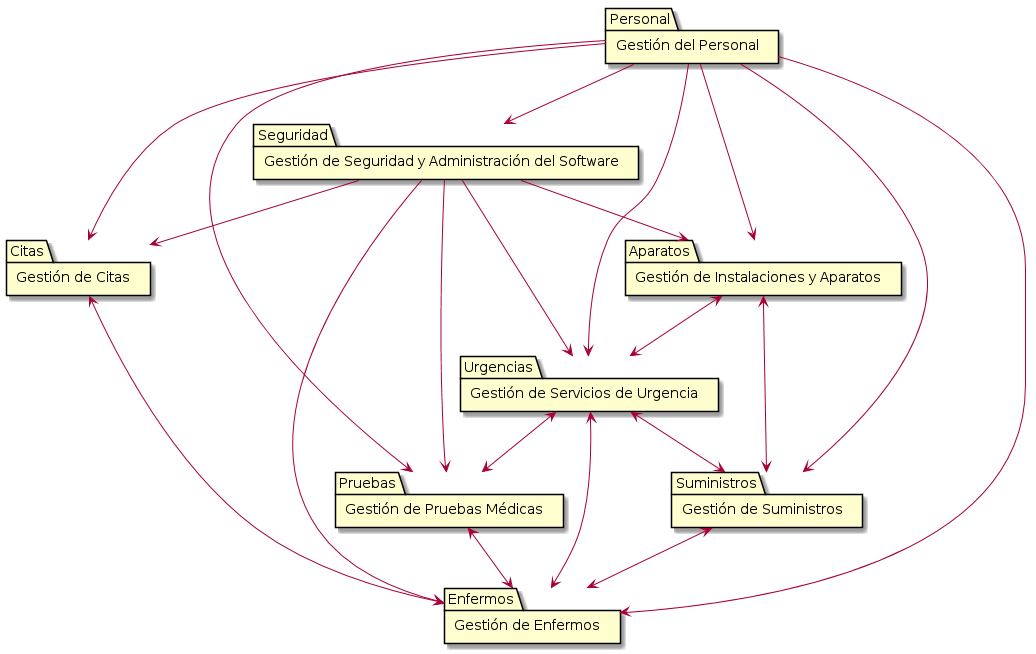
\includegraphics[scale=0.4]{DiagramaPaquetes}
	
	
\end{document}